\section{Time Series}
\frame{\sectionpage}

\begin{frame}[fragile]{Assessing time trends}
  
  To start, assess time trends using:
  
  \begin{itemize}
  \item correlation methods:
    \begin{itemize}
    \item regular Pearson correlation
    \item Mann-Kendall
    \end{itemize}
    

  \item regression methods:
    \begin{itemize}
    \item regression slope
    \item Theil-Sen slope
    \end{itemize}
  \end{itemize}
  
\end{frame}

\begin{frame}[fragile]{World mean temperatures}
  
  Since 1880:
  
\begin{knitrout}
\definecolor{shadecolor}{rgb}{0.969, 0.969, 0.969}\color{fgcolor}\begin{kframe}
\begin{alltt}
\hlstd{temp}\hlkwb{=}\hlkwd{read.csv}\hlstd{(}\hlstr{"temperature.csv"}\hlstd{)}
\hlkwd{head}\hlstd{(temp)}
\end{alltt}
\begin{verbatim}
##   X       Year temperature year
## 1 1 1880-12-31       13.72 1880
## 2 2 1881-12-31       13.79 1881
## 3 3 1882-12-31       13.74 1882
## 4 4 1883-12-31       13.73 1883
## 5 5 1884-12-31       13.68 1884
## 6 6 1885-12-31       13.68 1885
\end{verbatim}
\begin{alltt}
\hlkwd{attach}\hlstd{(temp)}
\end{alltt}
\end{kframe}
\end{knitrout}

\begin{knitrout}
\definecolor{shadecolor}{rgb}{0.969, 0.969, 0.969}\color{fgcolor}\begin{kframe}
\begin{alltt}
\hlkwd{plot}\hlstd{(temperature}\hlopt{~}\hlstd{year,}\hlkwc{type}\hlstd{=}\hlstr{"l"}\hlstd{)}
\hlkwd{lines}\hlstd{(}\hlkwd{lowess}\hlstd{(temperature}\hlopt{~}\hlstd{year))}
\end{alltt}
\end{kframe}
\end{knitrout}

\end{frame}

\begin{frame}[fragile]{Time plot}
  
\begin{knitrout}
\definecolor{shadecolor}{rgb}{0.969, 0.969, 0.969}\color{fgcolor}
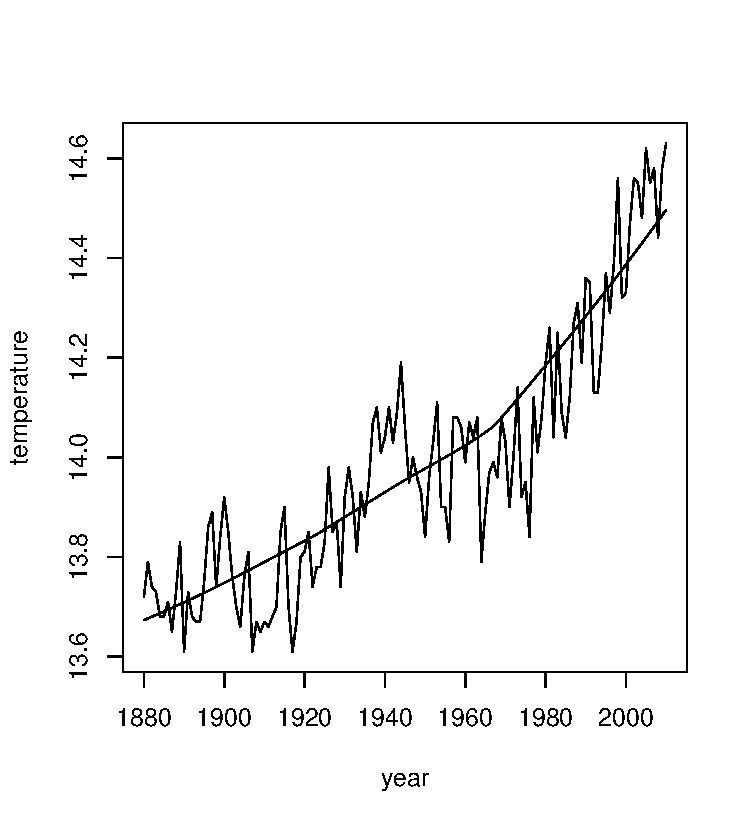
\includegraphics[width=\maxwidth]{figure/kahdkjheoiu-1} 

\end{knitrout}
  
\end{frame}


\begin{frame}[fragile]{Examining trend: Pearson}
  
  \begin{itemize}
  \item Pearson (regular) correlation, tests for \emph{linear} trend
    with \emph{normal} residuals (no outliers):
{\small
\begin{knitrout}
\definecolor{shadecolor}{rgb}{0.969, 0.969, 0.969}\color{fgcolor}\begin{kframe}
\begin{alltt}
\hlkwd{cor.test}\hlstd{(temperature,year)}
\end{alltt}
\begin{verbatim}
## 
## 	Pearson's product-moment correlation
## 
## data:  temperature and year
## t = 19.996, df = 129, p-value < 2.2e-16
## alternative hypothesis: true correlation is not equal to 0
## 95 percent confidence interval:
##  0.8203548 0.9059362
## sample estimates:
##       cor 
## 0.8695276
\end{verbatim}
\end{kframe}
\end{knitrout}
}
  \end{itemize}
  
\end{frame}

\begin{frame}[fragile]{Examining trend: Kendall \& Mann-Kendall}
  
  
  \begin{itemize}
\item Kendall (nonparametric) correlation, tests for \emph{monotone}
  trend, resistant to outliers:

{\small  
\begin{knitrout}
\definecolor{shadecolor}{rgb}{0.969, 0.969, 0.969}\color{fgcolor}\begin{kframe}
\begin{alltt}
\hlkwd{cor.test}\hlstd{(temperature,year,}\hlkwc{method}\hlstd{=}\hlstr{"kendall"}\hlstd{)}
\end{alltt}
\begin{verbatim}
## 
## 	Kendall's rank correlation tau
## 
## data:  temperature and year
## z = 11.776, p-value < 2.2e-16
## alternative hypothesis: true tau is not equal to 0
## sample estimates:
##       tau 
## 0.6992574
\end{verbatim}
\end{kframe}
\end{knitrout}
}

\item Another way to do this: Mann-Kendall correlation (Kendall test
  against \emph{time} or \emph{order}:
 
{\small  
\begin{knitrout}
\definecolor{shadecolor}{rgb}{0.969, 0.969, 0.969}\color{fgcolor}\begin{kframe}
\begin{alltt}
\hlkwd{library}\hlstd{(Kendall)}
\end{alltt}


{\ttfamily\noindent\bfseries\color{errorcolor}{\#\# Error in library(Kendall): there is no package called 'Kendall'}}\begin{alltt}
\hlkwd{MannKendall}\hlstd{(temperature)}
\end{alltt}


{\ttfamily\noindent\bfseries\color{errorcolor}{\#\# Error in eval(expr, envir, enclos): could not find function "{}MannKendall"{}}}\end{kframe}
\end{knitrout}
}
  \end{itemize}
\end{frame}


\begin{frame}[fragile]{Rate of change}

  \begin{itemize}
  \item Ordinary regression against time:
{\small
\begin{knitrout}
\definecolor{shadecolor}{rgb}{0.969, 0.969, 0.969}\color{fgcolor}\begin{kframe}
\begin{alltt}
\hlstd{temp.lm}\hlkwb{=}\hlkwd{lm}\hlstd{(temperature}\hlopt{~}\hlstd{year)}
\hlkwd{summary}\hlstd{(temp.lm)}\hlopt{$}\hlstd{coefficients}
\end{alltt}
\begin{verbatim}
##                Estimate   Std. Error   t value     Pr(>|t|)
## (Intercept) 2.579419741 0.5703983669  4.522137 1.370671e-05
## year        0.005863129 0.0002932085 19.996448 2.416159e-41
\end{verbatim}
\end{kframe}
\end{knitrout}
}
\item Slope about 0.0059 per year, 0.8
  degrees over 
  time period of study.
  \end{itemize}
  
\end{frame}

\begin{frame}[fragile]{Theil-Sen slope}
  \begin{itemize}
  \item Slope that assumes linearity, but not affected by outliers:
\begin{knitrout}
\definecolor{shadecolor}{rgb}{0.969, 0.969, 0.969}\color{fgcolor}\begin{kframe}
\begin{alltt}
\hlkwd{library}\hlstd{(zyp)}
\end{alltt}


{\ttfamily\noindent\bfseries\color{errorcolor}{\#\# Error in library(zyp): there is no package called 'zyp'}}\begin{alltt}
\hlstd{temp.zs}\hlkwb{=}\hlkwd{zyp.sen}\hlstd{(temperature}\hlopt{~}\hlstd{year,}\hlkwc{data}\hlstd{=temp)}
\end{alltt}


{\ttfamily\noindent\bfseries\color{errorcolor}{\#\# Error in eval(expr, envir, enclos): could not find function "{}zyp.sen"{}}}\begin{alltt}
\hlstd{temp.zs}\hlopt{$}\hlstd{coefficients}
\end{alltt}


{\ttfamily\noindent\bfseries\color{errorcolor}{\#\# Error in eval(expr, envir, enclos): object 'temp.zs' not found}}\end{kframe}
\end{knitrout}
\item Or:
\begin{knitrout}
\definecolor{shadecolor}{rgb}{0.969, 0.969, 0.969}\color{fgcolor}\begin{kframe}
\begin{alltt}
\hlstd{z}\hlkwb{=}\hlkwd{zyp.trend.vector}\hlstd{(temperature)}
\end{alltt}


{\ttfamily\noindent\bfseries\color{errorcolor}{\#\# Error in eval(expr, envir, enclos): could not find function "{}zyp.trend.vector"{}}}\begin{alltt}
\hlstd{z[}\hlstr{"trend"}\hlstd{]}
\end{alltt}


{\ttfamily\noindent\bfseries\color{errorcolor}{\#\# Error in eval(expr, envir, enclos): object 'z' not found}}\begin{alltt}
\hlkwd{detach}\hlstd{(temp)}
\end{alltt}
\end{kframe}
\end{knitrout}
\item Doesn't need year.
\item Theil-Sen slope about 0.0057.
  \end{itemize}
  
\end{frame}

\begin{frame}[fragile]{Conclusions}
  
  \begin{itemize}
\item Linear regression slope is 0.005863
\item Theil-Sen slope is 0.005676
\item Very close.
\item Pearson correlation is 0.8675
\item Kendall correlation is 0.6993
\item Both correlations have P-value $< 2.2 \times 10^{-16}$. 
\item Kendall correlation smaller, but P-value equally significant
  (usually the case). 

\item \textbf{Successive values assumed independent, but probably not
    in actuality. To take care of dependence, need actual time series methods.}
  \end{itemize}
  
\end{frame}

\begin{frame}[fragile]{The Monarchs of England}
  \begin{itemize}
  \item Age at death of Kings and Queens of England since William the
    Conqueror (1066):
\begin{knitrout}
\definecolor{shadecolor}{rgb}{0.969, 0.969, 0.969}\color{fgcolor}\begin{kframe}
\begin{alltt}
\hlstd{kings}\hlkwb{=}\hlkwd{read.table}\hlstd{(}\hlstr{"kings.txt"}\hlstd{,}\hlkwc{header}\hlstd{=F)}
\hlkwd{head}\hlstd{(kings)}
\end{alltt}
\begin{verbatim}
##   V1
## 1 60
## 2 43
## 3 67
## 4 50
## 5 56
## 6 42
\end{verbatim}
\end{kframe}
\end{knitrout}

\item Data in one long column \texttt{V1}.
\item Turn into time series \texttt{ts} object.
  
\begin{knitrout}
\definecolor{shadecolor}{rgb}{0.969, 0.969, 0.969}\color{fgcolor}\begin{kframe}
\begin{alltt}
\hlstd{kings.ts}\hlkwb{=}\hlkwd{ts}\hlstd{(kings)}
\end{alltt}
\end{kframe}
\end{knitrout}

  \end{itemize}
\end{frame}

\begin{frame}[fragile]{Plotting a time series}
  
\begin{knitrout}
\definecolor{shadecolor}{rgb}{0.969, 0.969, 0.969}\color{fgcolor}\begin{kframe}
\begin{alltt}
\hlkwd{plot}\hlstd{(kings.ts) ;} \hlkwd{lines}\hlstd{(}\hlkwd{lowess}\hlstd{(kings.ts))}
\end{alltt}
\end{kframe}
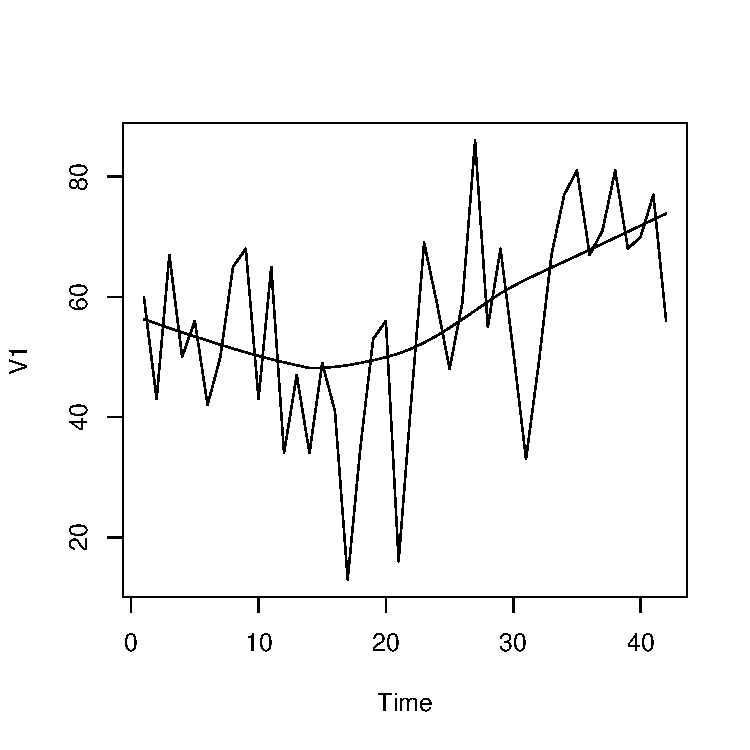
\includegraphics[width=\maxwidth]{figure/raghib-1} 

\end{knitrout}
  
\end{frame}

\begin{frame}[fragile]{Comments}
  
  \begin{itemize}
  \item ``Time'' here order of monarch from William the Conqueror (1)
    to George VI (42).
  \item Slightly increasing trend of age at death
  \item but lots of irregularity.
  \end{itemize}
  
\end{frame}

\begin{frame}[fragile]{Stationarity}
  
  \begin{itemize}
  \item Time series stationary if:
    \begin{itemize}
    \item mean constant over time
    \item variability constant over time and not dependent on mean.
    \end{itemize}
  \item Kings series:
    \begin{itemize}
    \item non-constant mean
    \item constant (?) variability
    \item not stationary.
    \end{itemize}
  \item Fix stationarity by taking differences: 2nd minus 1st, 3rd
    minus 2nd, etc:
\begin{knitrout}
\definecolor{shadecolor}{rgb}{0.969, 0.969, 0.969}\color{fgcolor}\begin{kframe}
\begin{alltt}
\hlstd{kings.diff.ts}\hlkwb{=}\hlkwd{diff}\hlstd{(kings.ts)}
\end{alltt}
\end{kframe}
\end{knitrout}
  \end{itemize}
  
\end{frame}


\begin{frame}[fragile]{Did differencing fix stationarity? Yes.}
  
\begin{knitrout}
\definecolor{shadecolor}{rgb}{0.969, 0.969, 0.969}\color{fgcolor}\begin{kframe}
\begin{alltt}
\hlkwd{plot}\hlstd{(kings.diff.ts,}\hlkwc{main}\hlstd{=}\hlstr{"Kings series, differenced"}\hlstd{)}
\hlkwd{lines}\hlstd{(}\hlkwd{lowess}\hlstd{(kings.diff.ts))}
\end{alltt}
\end{kframe}
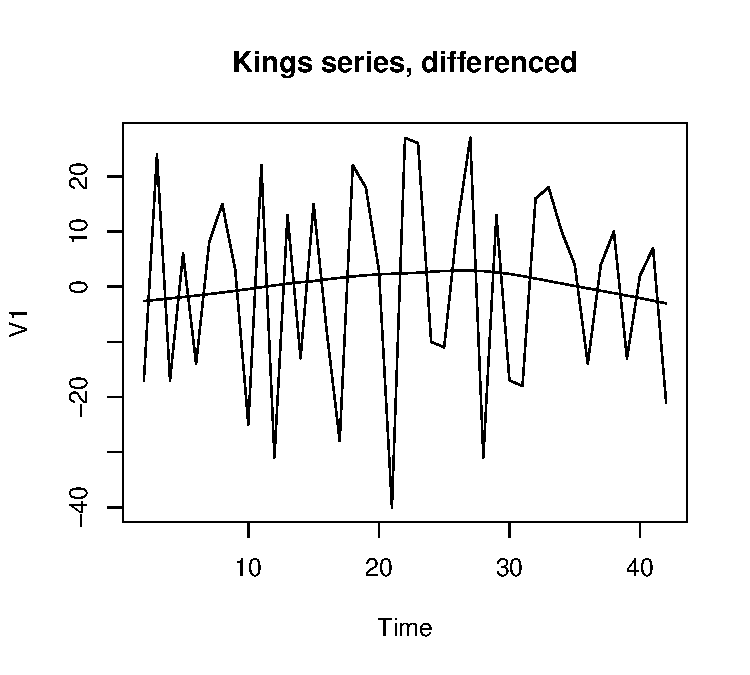
\includegraphics[width=\maxwidth]{figure/lsjahjsh-1} 

\end{knitrout}
  
\end{frame}

\begin{frame}[fragile]{Births per month in New York City}
  \begin{itemize}
  \item From  January 1946 to December 1959:
\begin{knitrout}
\definecolor{shadecolor}{rgb}{0.969, 0.969, 0.969}\color{fgcolor}\begin{kframe}
\begin{alltt}
\hlstd{ny}\hlkwb{=}\hlkwd{read.table}\hlstd{(}\hlstr{"nybirths.txt"}\hlstd{,}\hlkwc{header}\hlstd{=F)}
\hlstd{ny.ts}\hlkwb{=}\hlkwd{ts}\hlstd{(ny,}\hlkwc{freq}\hlstd{=}\hlnum{12}\hlstd{,}\hlkwc{start}\hlstd{=}\hlkwd{c}\hlstd{(}\hlnum{1946}\hlstd{,}\hlnum{1}\hlstd{))}
\end{alltt}
\end{kframe}
\end{knitrout}
\item Note extras on `ts`:
  \begin{itemize}
\item Time period is 1 year
\item 12 observations per year (monthly) in `freq`
\item First observation is 1st month of 1946 in `start`
  \end{itemize}
  \end{itemize}
\end{frame}


\begin{frame}[fragile]{Printing formats nicely}
  
{\tiny
\begin{knitrout}
\definecolor{shadecolor}{rgb}{0.969, 0.969, 0.969}\color{fgcolor}\begin{kframe}
\begin{alltt}
\hlstd{ny.ts}
\end{alltt}
\begin{verbatim}
##         Jan    Feb    Mar    Apr    May    Jun    Jul    Aug    Sep    Oct    Nov    Dec
## 1946 26.663 23.598 26.931 24.740 25.806 24.364 24.477 23.901 23.175 23.227 21.672 21.870
## 1947 21.439 21.089 23.709 21.669 21.752 20.761 23.479 23.824 23.105 23.110 21.759 22.073
## 1948 21.937 20.035 23.590 21.672 22.222 22.123 23.950 23.504 22.238 23.142 21.059 21.573
## 1949 21.548 20.000 22.424 20.615 21.761 22.874 24.104 23.748 23.262 22.907 21.519 22.025
## 1950 22.604 20.894 24.677 23.673 25.320 23.583 24.671 24.454 24.122 24.252 22.084 22.991
## 1951 23.287 23.049 25.076 24.037 24.430 24.667 26.451 25.618 25.014 25.110 22.964 23.981
## 1952 23.798 22.270 24.775 22.646 23.988 24.737 26.276 25.816 25.210 25.199 23.162 24.707
## 1953 24.364 22.644 25.565 24.062 25.431 24.635 27.009 26.606 26.268 26.462 25.246 25.180
## 1954 24.657 23.304 26.982 26.199 27.210 26.122 26.706 26.878 26.152 26.379 24.712 25.688
## 1955 24.990 24.239 26.721 23.475 24.767 26.219 28.361 28.599 27.914 27.784 25.693 26.881
## 1956 26.217 24.218 27.914 26.975 28.527 27.139 28.982 28.169 28.056 29.136 26.291 26.987
## 1957 26.589 24.848 27.543 26.896 28.878 27.390 28.065 28.141 29.048 28.484 26.634 27.735
## 1958 27.132 24.924 28.963 26.589 27.931 28.009 29.229 28.759 28.405 27.945 25.912 26.619
## 1959 26.076 25.286 27.660 25.951 26.398 25.565 28.865 30.000 29.261 29.012 26.992 27.897
\end{verbatim}
\end{kframe}
\end{knitrout}
}
  
\end{frame}

\begin{frame}[fragile]{Time plot: extra pattern}
  
\begin{knitrout}
\definecolor{shadecolor}{rgb}{0.969, 0.969, 0.969}\color{fgcolor}\begin{kframe}
\begin{alltt}
\hlkwd{plot}\hlstd{(ny.ts)}
\end{alltt}
\end{kframe}
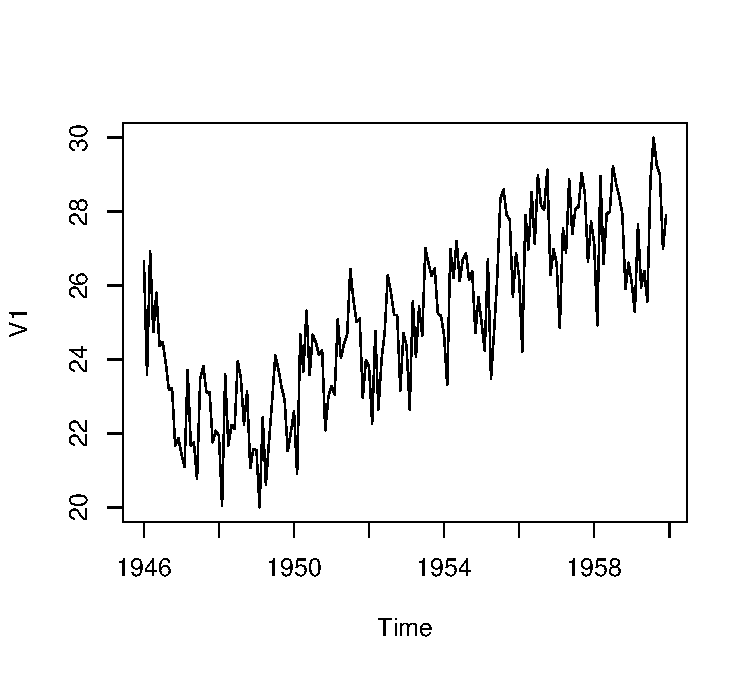
\includegraphics[width=\maxwidth]{figure/akjsalkasl-1} 

\end{knitrout}
  
\end{frame}

\begin{frame}[fragile]{Comments on time plot}
  
  \begin{itemize}
\item steady increase
\item repeating pattern each year (seasonal component).
\item Not stationary.
  \end{itemize}
  
\end{frame}

\begin{frame}[fragile]{Differencing the New York births: does it help?}
  
Stationary, but regular spikes:  
  
\begin{knitrout}
\definecolor{shadecolor}{rgb}{0.969, 0.969, 0.969}\color{fgcolor}\begin{kframe}
\begin{alltt}
\hlstd{ny.diff.ts}\hlkwb{=}\hlkwd{diff}\hlstd{(ny.ts)}
\hlkwd{plot}\hlstd{(ny.diff.ts)}
\hlkwd{lines}\hlstd{(}\hlkwd{lowess}\hlstd{(ny.diff.ts))}
\end{alltt}
\end{kframe}
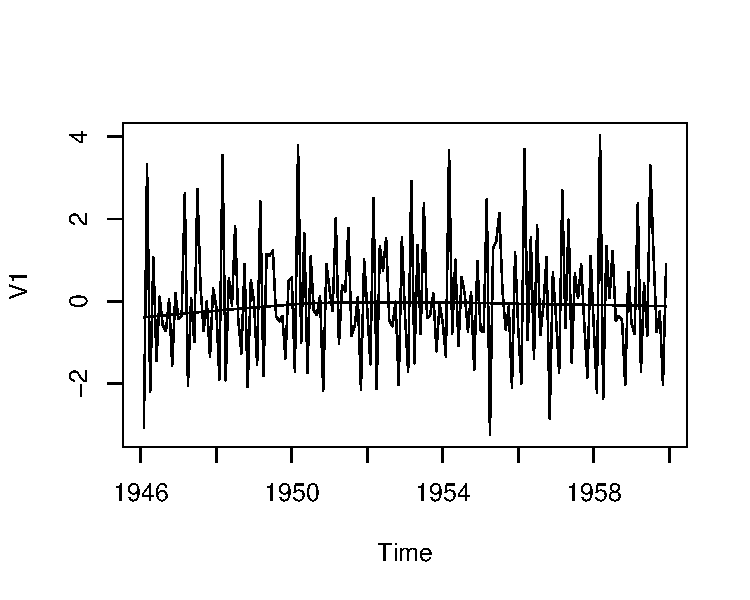
\includegraphics[width=\maxwidth]{figure/sklsalhsa-1} 

\end{knitrout}
  
\end{frame}

\begin{frame}[fragile]{Visual: decomposing seasonal time series}
  
\begin{knitrout}
\definecolor{shadecolor}{rgb}{0.969, 0.969, 0.969}\color{fgcolor}\begin{kframe}
\begin{alltt}
\hlstd{ny.d}\hlkwb{=}\hlkwd{decompose}\hlstd{(ny.ts)}
\hlkwd{plot}\hlstd{(ny.d)}
\end{alltt}
\end{kframe}
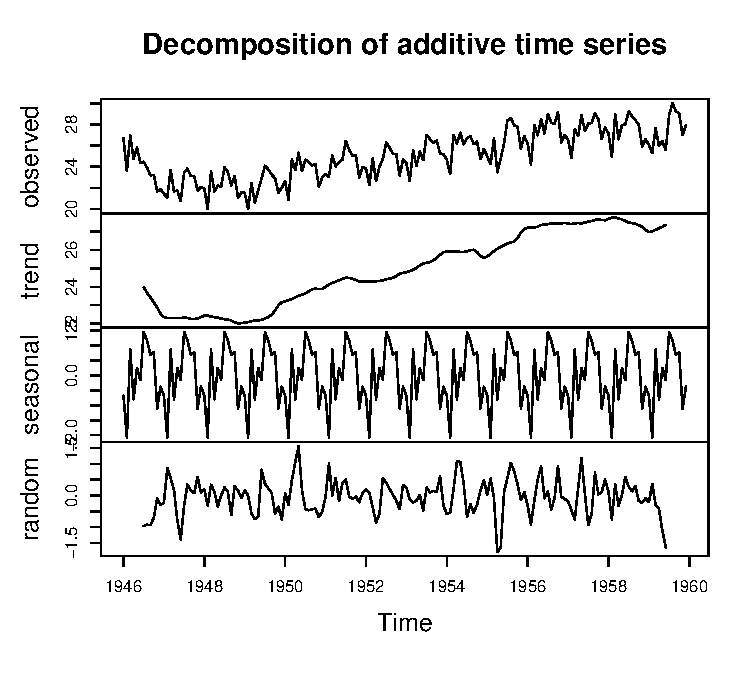
\includegraphics[width=\maxwidth]{figure/askjasklslak-1} 

\end{knitrout}
  
\end{frame}

\begin{frame}{Decomposition bits}
  
  \begin{itemize}
\item original series
\item just the trend, going steadily up (except at the start)
\item a "seasonal" part: something that repeats every year (births
  lowest in Feb, highest in Jul).
\item random: what is left over ("residuals")
  \end{itemize}
  
\end{frame}


\begin{frame}[fragile]{Time series basics: white noise}
  
Independent random normal. Knowing one value tells you nothing about
the next.  ``Random'' process:



{\small
\begin{knitrout}
\definecolor{shadecolor}{rgb}{0.969, 0.969, 0.969}\color{fgcolor}\begin{kframe}
\begin{alltt}
\hlstd{wn}\hlkwb{=}\hlkwd{rnorm}\hlstd{(}\hlnum{100}\hlstd{)}
\hlstd{wn.ts}\hlkwb{=}\hlkwd{ts}\hlstd{(wn)}
\hlkwd{plot}\hlstd{(wn.ts)}
\end{alltt}
\end{kframe}
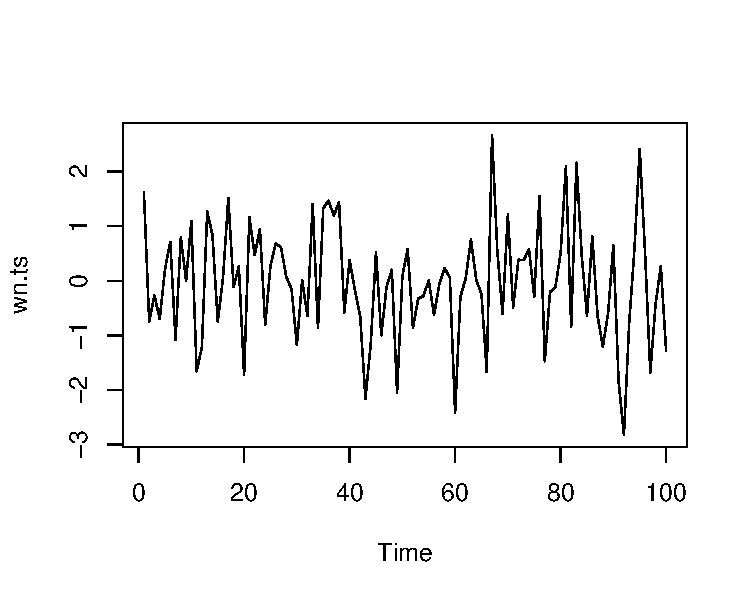
\includegraphics[width=\maxwidth]{figure/ternana-1} 

\end{knitrout}
}
  
  
\end{frame}

\begin{frame}[fragile]{Lagging a time series}

Moving a time series one (or more) steps back in time:

\begin{knitrout}
\definecolor{shadecolor}{rgb}{0.969, 0.969, 0.969}\color{fgcolor}\begin{kframe}
\begin{alltt}
\hlstd{x}\hlkwb{=}\hlkwd{rnorm}\hlstd{(}\hlnum{5}\hlstd{)}
\hlstd{x.1}\hlkwb{=}\hlkwd{c}\hlstd{(}\hlnum{NA}\hlstd{,x)}
\hlstd{x.0}\hlkwb{=}\hlkwd{c}\hlstd{(x,}\hlnum{NA}\hlstd{)}
\hlkwd{cbind}\hlstd{(x.0,x.1)}
\end{alltt}
\begin{verbatim}
##              x.0         x.1
## [1,] -2.03609485          NA
## [2,] -0.57861580 -2.03609485
## [3,]  0.60836463 -0.57861580
## [4,]  0.11803343  0.60836463
## [5,]  0.05634432  0.11803343
## [6,]          NA  0.05634432
\end{verbatim}
\end{kframe}
\end{knitrout}

Have to glue `NA` onto \emph{both} ends to keep series same length.

\end{frame}

\begin{frame}[fragile]{Lagging white noise}
  
\begin{knitrout}
\definecolor{shadecolor}{rgb}{0.969, 0.969, 0.969}\color{fgcolor}\begin{kframe}
\begin{alltt}
\hlstd{wn.1}\hlkwb{=}\hlkwd{c}\hlstd{(}\hlnum{NA}\hlstd{,wn) ; wn.0}\hlkwb{=}\hlkwd{c}\hlstd{(wn,}\hlnum{NA}\hlstd{) ;} \hlkwd{plot}\hlstd{(wn.1,wn.0)}
\end{alltt}
\end{kframe}
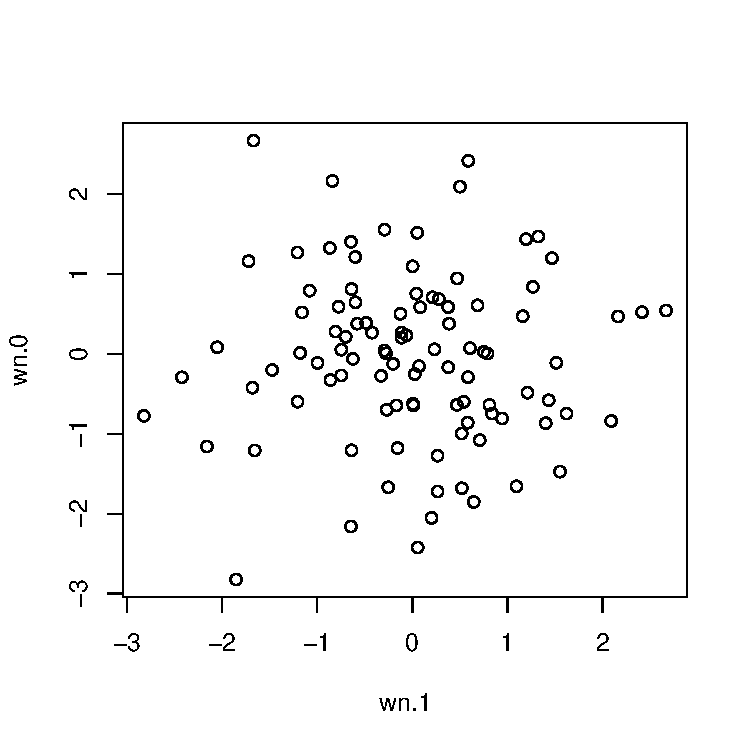
\includegraphics[width=\maxwidth]{figure/ipswich-1} 

\end{knitrout}
  
\end{frame}


\begin{frame}[fragile]{Correlation with lagged series}
  \begin{itemize}
  \item If you know about white noise at one time point, you know
    \emph{nothing} about it at the next. This is shown by the scatterplot
    and the correlation:
\begin{knitrout}
\definecolor{shadecolor}{rgb}{0.969, 0.969, 0.969}\color{fgcolor}\begin{kframe}
\begin{alltt}
\hlkwd{cor}\hlstd{(wn.1,wn.0,}\hlkwc{use}\hlstd{=}\hlstr{"c"}\hlstd{)}
\end{alltt}
\begin{verbatim}
## [1] -0.01676257
\end{verbatim}
\end{kframe}
\end{knitrout}
  \item On the other hand, this:
\begin{knitrout}
\definecolor{shadecolor}{rgb}{0.969, 0.969, 0.969}\color{fgcolor}\begin{kframe}
\begin{alltt}
\hlstd{kings.1}\hlkwb{=}\hlkwd{c}\hlstd{(}\hlnum{NA}\hlstd{,kings.ts)}
\hlstd{kings.0}\hlkwb{=}\hlkwd{c}\hlstd{(kings.ts,}\hlnum{NA}\hlstd{)}
\hlkwd{cor}\hlstd{(kings.1,kings.0,}\hlkwc{use}\hlstd{=}\hlstr{"c"}\hlstd{)}
\end{alltt}
\begin{verbatim}
## [1] 0.4009919
\end{verbatim}
\end{kframe}
\end{knitrout}

\item If one value larger, the next value (a bit) more likely to be larger. 


  \end{itemize}
\end{frame}

\begin{frame}[fragile]{Plot of series vs. lagged series for kings data}
  
\begin{knitrout}
\definecolor{shadecolor}{rgb}{0.969, 0.969, 0.969}\color{fgcolor}\begin{kframe}
\begin{alltt}
\hlkwd{plot}\hlstd{(kings.1,kings.0)}
\end{alltt}
\end{kframe}
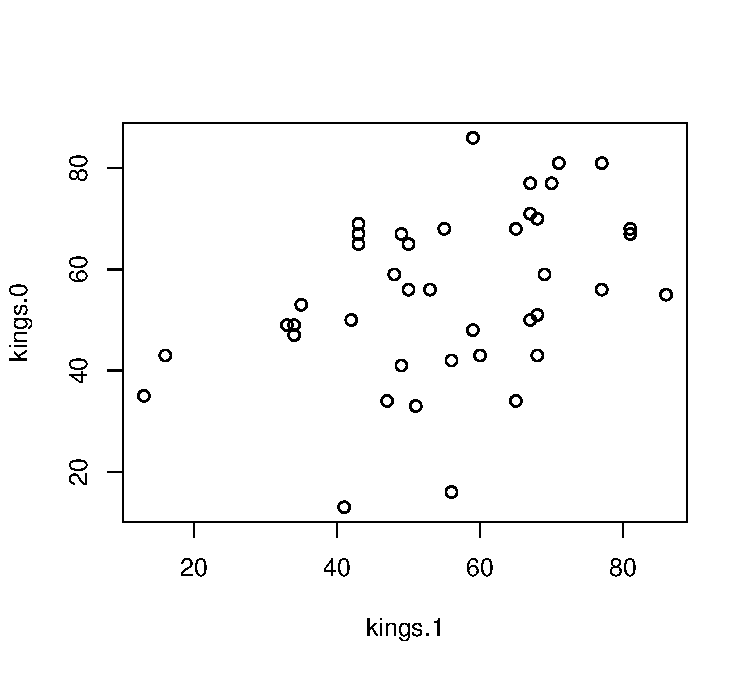
\includegraphics[width=\maxwidth]{figure/partington-1} 

\end{knitrout}
  
\end{frame}

\begin{frame}[fragile]{Two steps back:}
  
\begin{knitrout}
\definecolor{shadecolor}{rgb}{0.969, 0.969, 0.969}\color{fgcolor}\begin{kframe}
\begin{alltt}
\hlcom{# one step back}
\hlkwd{cor}\hlstd{(kings.1,kings.0,}\hlkwc{use}\hlstd{=}\hlstr{"c"}\hlstd{)}
\end{alltt}
\begin{verbatim}
## [1] 0.4009919
\end{verbatim}
\begin{alltt}
\hlcom{# one step plus one more}
\hlstd{kings.2}\hlkwb{=}\hlkwd{c}\hlstd{(}\hlnum{NA}\hlstd{,kings.1)}
\hlstd{kings.0}\hlkwb{=}\hlkwd{c}\hlstd{(kings.0,}\hlnum{NA}\hlstd{)}
\hlkwd{cor}\hlstd{(kings.0,kings.2,}\hlkwc{use}\hlstd{=}\hlstr{"c"}\hlstd{)}
\end{alltt}
\begin{verbatim}
## [1] 0.245676
\end{verbatim}
\end{kframe}
\end{knitrout}

Still a correlation two steps back, but smaller.

  
\end{frame}


\begin{frame}[fragile]{Autocorrelation}
  
  \begin{itemize}
  \item Correlation of time series with \emph{itself} one, two,... time
    steps back is useful idea, called \textbf{autocorrelation}. Make a plot
    of it with \texttt{acf}. White noise: 
\begin{knitrout}
\definecolor{shadecolor}{rgb}{0.969, 0.969, 0.969}\color{fgcolor}\begin{kframe}
\begin{alltt}
\hlkwd{acf}\hlstd{(wn.ts)}
\end{alltt}
\end{kframe}
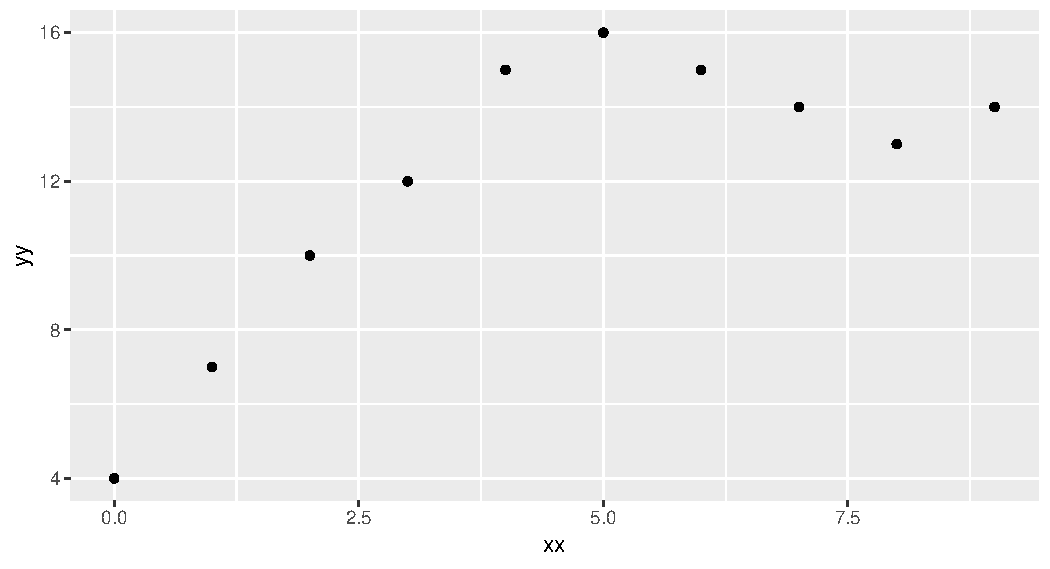
\includegraphics[width=\maxwidth]{figure/unnamed-chunk-18-1} 

\end{knitrout}
  \end{itemize}
  
\end{frame}

\begin{frame}[fragile]{Comments}
  
  \begin{itemize}
\item No autocorrelations beyond chance, anywhere. Ignore 0.

\item Autocorrelations work best on \emph{stationary} series.
  \end{itemize}
  
\end{frame}


\begin{frame}[fragile]{Kings, differenced}
  
\begin{knitrout}
\definecolor{shadecolor}{rgb}{0.969, 0.969, 0.969}\color{fgcolor}\begin{kframe}
\begin{alltt}
\hlkwd{acf}\hlstd{(kings.diff.ts)}
\end{alltt}
\end{kframe}
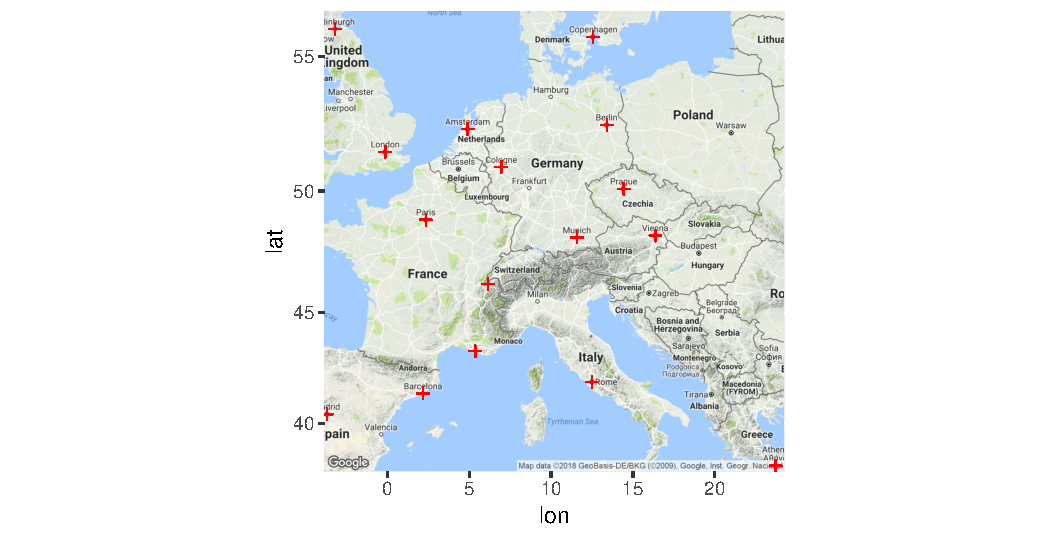
\includegraphics[width=\maxwidth]{figure/unnamed-chunk-19-1} 

\end{knitrout}
  
\end{frame}

\begin{frame}{Comments on autocorrelations of kings series}
  

Negative autocorrelation at lag 1, nothing beyond that. 

\begin{itemize}
\item If one value of differenced series positive, next one most
  likely negative. 
\item If one king lives longer than predecessor, next one likely lives shorter.

\end{itemize}
  
  
\end{frame}

\begin{frame}[fragile]{NY births, differenced}
  
\begin{knitrout}
\definecolor{shadecolor}{rgb}{0.969, 0.969, 0.969}\color{fgcolor}\begin{kframe}
\begin{alltt}
\hlkwd{acf}\hlstd{(ny.diff.ts,}\hlkwc{main}\hlstd{=}\hlstr{"NY births differenced"}\hlstd{)}
\end{alltt}
\end{kframe}
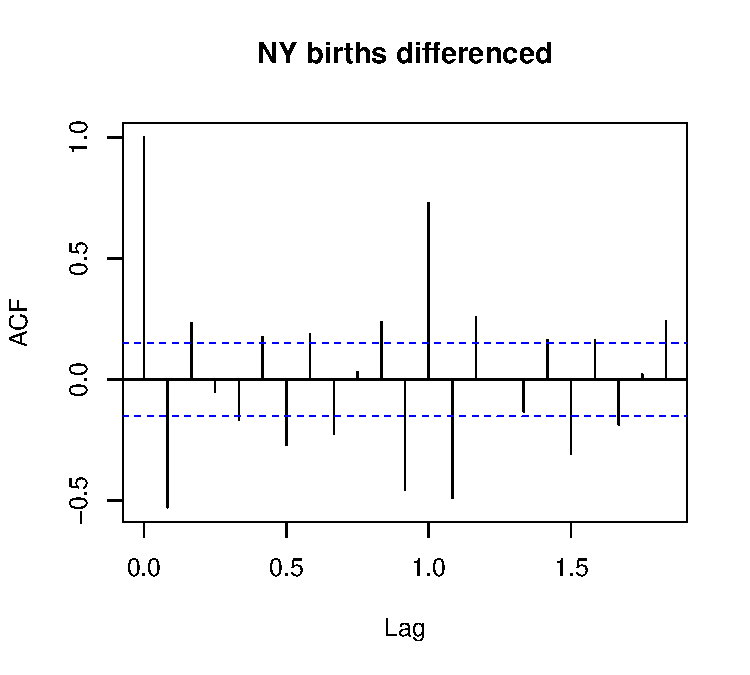
\includegraphics[width=\maxwidth]{figure/cesena-1} 

\end{knitrout}
  
\end{frame}

\begin{frame}[fragile]{Comments}

  Lots of stuff:

  \begin{itemize}
\item large positive autocorrelation at 1.0 years (July one year like July last year)
\item large negative autocorrelation at 1 month.
\item smallish but significant negative autocorrelation at 0.5 year = 6 months.
\item Other stuff -- complicated.

  \end{itemize}
  
\end{frame}

\begin{frame}[fragile]{Souvenir sales}
  
Monthly sales for a beach souvenir shop in Queensland, Australia:

\begin{knitrout}
\definecolor{shadecolor}{rgb}{0.969, 0.969, 0.969}\color{fgcolor}\begin{kframe}
\begin{alltt}
\hlstd{souv}\hlkwb{=}\hlkwd{read.table}\hlstd{(}\hlstr{"souvenir.txt"}\hlstd{,}\hlkwc{header}\hlstd{=F)}
\hlstd{souv.ts}\hlkwb{=}\hlkwd{ts}\hlstd{(souv,}\hlkwc{frequency}\hlstd{=}\hlnum{12}\hlstd{,}\hlkwc{start}\hlstd{=}\hlnum{1987}\hlstd{)}
\end{alltt}
\end{kframe}
\end{knitrout}

{\tiny
\begin{knitrout}
\definecolor{shadecolor}{rgb}{0.969, 0.969, 0.969}\color{fgcolor}\begin{kframe}
\begin{alltt}
\hlstd{souv.ts}
\end{alltt}
\begin{verbatim}
##            Jan       Feb       Mar       Apr       May       Jun       Jul       Aug
## 1987   1664.81   2397.53   2840.71   3547.29   3752.96   3714.74   4349.61   3566.34
## 1988   2499.81   5198.24   7225.14   4806.03   5900.88   4951.34   6179.12   4752.15
## 1989   4717.02   5702.63   9957.58   5304.78   6492.43   6630.80   7349.62   8176.62
## 1990   5921.10   5814.58  12421.25   6369.77   7609.12   7224.75   8121.22   7979.25
## 1991   4826.64   6470.23   9638.77   8821.17   8722.37  10209.48  11276.55  12552.22
## 1992   7615.03   9849.69  14558.40  11587.33   9332.56  13082.09  16732.78  19888.61
## 1993  10243.24  11266.88  21826.84  17357.33  15997.79  18601.53  26155.15  28586.52
##            Sep       Oct       Nov       Dec
## 1987   5021.82   6423.48   7600.60  19756.21
## 1988   5496.43   5835.10  12600.08  28541.72
## 1989   8573.17   9690.50  15151.84  34061.01
## 1990   8093.06   8476.70  17914.66  30114.41
## 1991  11637.39  13606.89  21822.11  45060.69
## 1992  23933.38  25391.35  36024.80  80721.71
## 1993  30505.41  30821.33  46634.38 104660.67
\end{verbatim}
\end{kframe}
\end{knitrout}
}

\end{frame}

\begin{frame}[fragile]{Plot of souvenir sales}
  
\begin{knitrout}
\definecolor{shadecolor}{rgb}{0.969, 0.969, 0.969}\color{fgcolor}\begin{kframe}
\begin{alltt}
\hlkwd{plot}\hlstd{(souv.ts)}
\end{alltt}
\end{kframe}
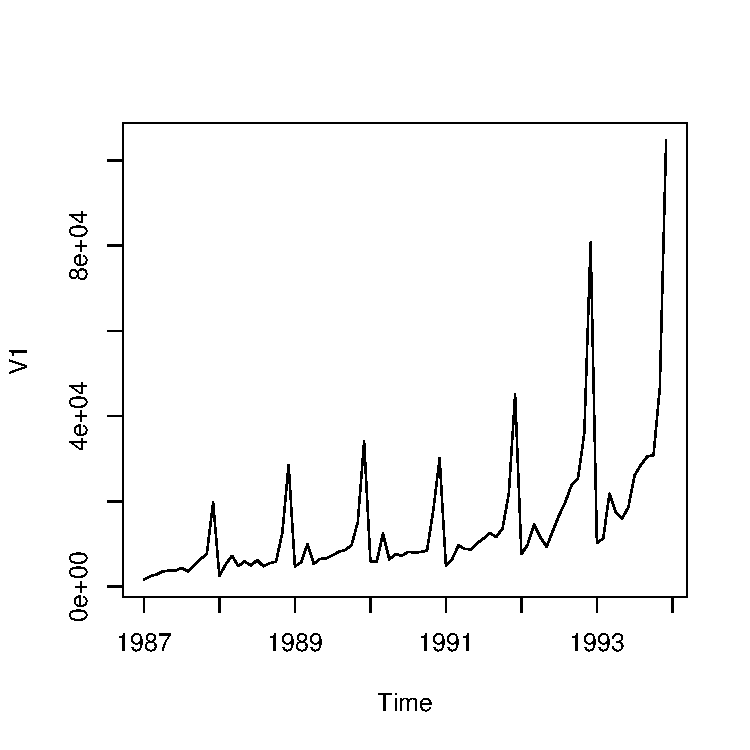
\includegraphics[width=\maxwidth]{figure/fiorentina-1} 

\end{knitrout}
  
\end{frame}

\begin{frame}[fragile]{Comments}

Several problems:

\begin{itemize}
\item Mean goes up over time
\item Variability gets larger as mean gets larger
\item Not stationary
\end{itemize}
  
\end{frame}

\begin{frame}[fragile]{Problem-fixing}
  
Fix non-constant variability first by taking logs:

\begin{knitrout}
\definecolor{shadecolor}{rgb}{0.969, 0.969, 0.969}\color{fgcolor}\begin{kframe}
\begin{alltt}
\hlstd{souv.log.ts}\hlkwb{=}\hlkwd{log}\hlstd{(souv.ts)}
\hlkwd{plot}\hlstd{(souv.log.ts)}
\end{alltt}
\end{kframe}
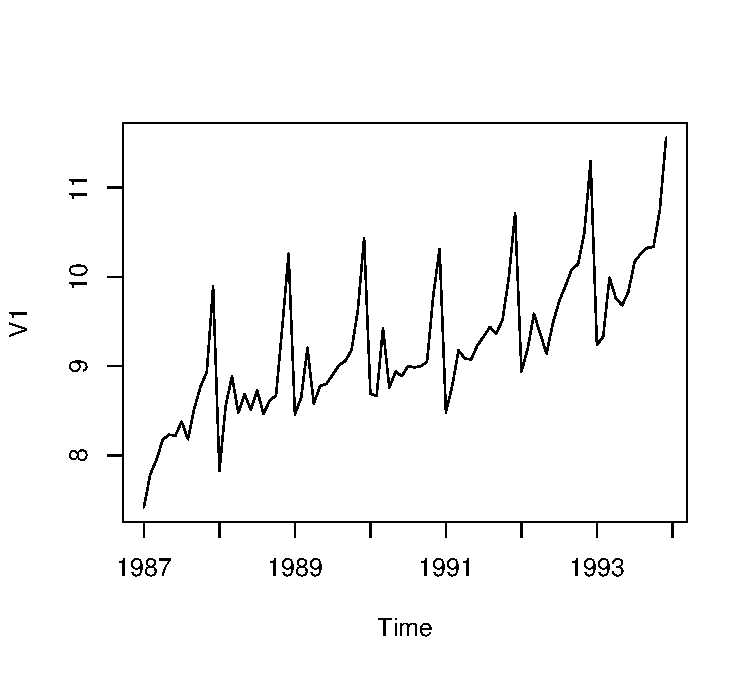
\includegraphics[width=\maxwidth]{figure/lupomartini-1} 

\end{knitrout}
  
\end{frame}

\begin{frame}[fragile]{Differencing}

  Mean still not constant, so try taking differences:
  
\begin{knitrout}
\definecolor{shadecolor}{rgb}{0.969, 0.969, 0.969}\color{fgcolor}\begin{kframe}
\begin{alltt}
\hlstd{souv.log.diff.ts}\hlkwb{=}\hlkwd{diff}\hlstd{(souv.log.ts)}
\hlkwd{plot}\hlstd{(souv.log.diff.ts)}
\end{alltt}
\end{kframe}
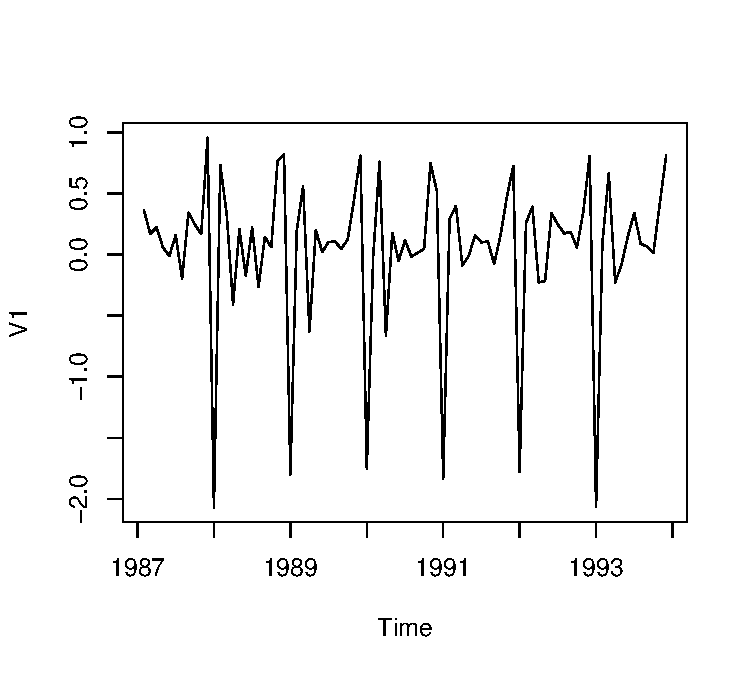
\includegraphics[width=\maxwidth]{figure/sambennedetese-1} 

\end{knitrout}
  
\end{frame}

\begin{frame}{Comments}
  
  \begin{itemize}
\item Now stationary
\item but clear seasonal effect.
  \end{itemize}
\end{frame}

\begin{frame}[fragile]{Decomposing to see the seasonal effect}
    
\begin{knitrout}
\definecolor{shadecolor}{rgb}{0.969, 0.969, 0.969}\color{fgcolor}\begin{kframe}
\begin{alltt}
\hlstd{souv.d}\hlkwb{=}\hlkwd{decompose}\hlstd{(souv.log.diff.ts)}
\hlkwd{plot}\hlstd{(souv.d)}
\end{alltt}
\end{kframe}
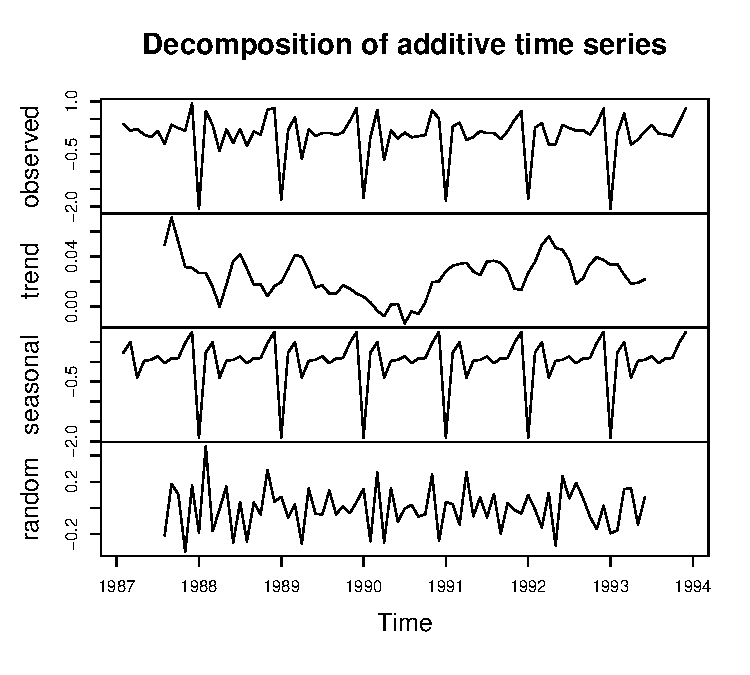
\includegraphics[width=\maxwidth]{figure/saklsdalkhdaskl-1} 

\end{knitrout}
  
\end{frame}

\begin{frame}[fragile]{Comments}
  
\emph{Big} drop in one month's differences. Look at seasonal component to
see which:  
  


{\small
\begin{knitrout}
\definecolor{shadecolor}{rgb}{0.969, 0.969, 0.969}\color{fgcolor}\begin{kframe}
\begin{alltt}
\hlkwd{round}\hlstd{(souv.d}\hlopt{$}\hlstd{seasonal,}\hlnum{2}\hlstd{)}
\end{alltt}
\begin{verbatim}
##        Jan   Feb   Mar   Apr   May   Jun   Jul   Aug   Sep
## 1987        0.23  0.49 -0.40  0.02  0.05  0.14 -0.04  0.09
## 1988 -1.90  0.23  0.49 -0.40  0.02  0.05  0.14 -0.04  0.09
## 1989 -1.90  0.23  0.49 -0.40  0.02  0.05  0.14 -0.04  0.09
## 1990 -1.90  0.23  0.49 -0.40  0.02  0.05  0.14 -0.04  0.09
## 1991 -1.90  0.23  0.49 -0.40  0.02  0.05  0.14 -0.04  0.09
## 1992 -1.90  0.23  0.49 -0.40  0.02  0.05  0.14 -0.04  0.09
## 1993 -1.90  0.23  0.49 -0.40  0.02  0.05  0.14 -0.04  0.09
##        Oct   Nov   Dec
## 1987  0.09  0.47  0.75
## 1988  0.09  0.47  0.75
## 1989  0.09  0.47  0.75
## 1990  0.09  0.47  0.75
## 1991  0.09  0.47  0.75
## 1992  0.09  0.47  0.75
## 1993  0.09  0.47  0.75
\end{verbatim}
\end{kframe}
\end{knitrout}
}
  
\end{frame}


\begin{frame}[fragile]{Autocorrelations}
  
  \begin{itemize}
\item Big positive autocorrelation at 1 year (strong seasonal effect)
\item Small negative autocorrelation at 1 and 2 months:
  
\begin{knitrout}
\definecolor{shadecolor}{rgb}{0.969, 0.969, 0.969}\color{fgcolor}\begin{kframe}
\begin{alltt}
\hlkwd{acf}\hlstd{(souv.log.diff.ts)}
\end{alltt}
\end{kframe}
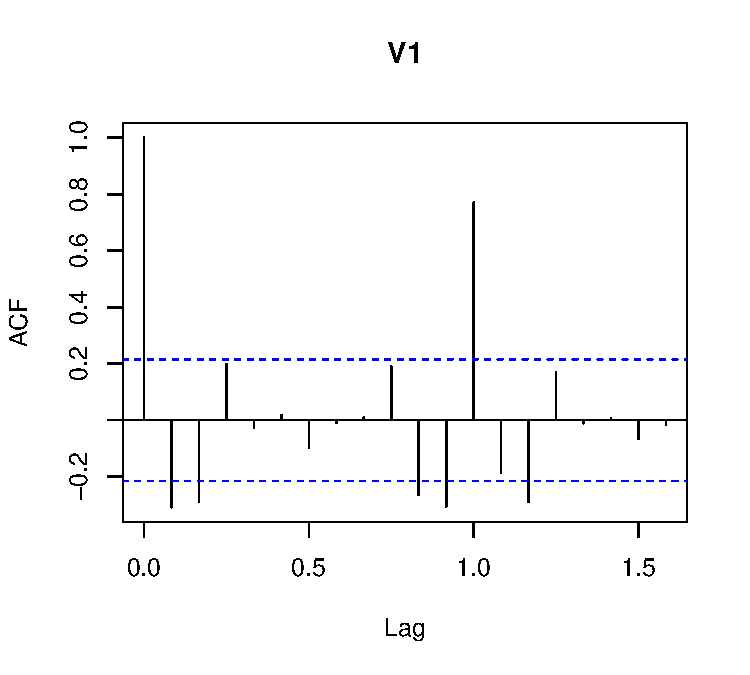
\includegraphics[width=\maxwidth]{figure/asjdhasjhsajkhdaskjhd-1} 

\end{knitrout}
  \end{itemize}
  
\end{frame}


\begin{frame}[fragile]{Moving average}
  
``Moving average'' or MA process captures idea of autocorrelations at
a few lags but not others. MA(1) process, with autocorrelation only at lag 1:

{\footnotesize
\begin{knitrout}
\definecolor{shadecolor}{rgb}{0.969, 0.969, 0.969}\color{fgcolor}\begin{kframe}
\begin{alltt}
\hlstd{e}\hlkwb{=}\hlkwd{rnorm}\hlstd{(}\hlnum{100}\hlstd{)}
\hlstd{y}\hlkwb{=}\hlkwd{numeric}\hlstd{(}\hlnum{0}\hlstd{)}
\hlstd{y[}\hlnum{1}\hlstd{]}\hlkwb{=}\hlnum{0}
\hlstd{beta}\hlkwb{=}\hlnum{1}
\hlkwa{for} \hlstd{(i} \hlkwa{in} \hlnum{2}\hlopt{:}\hlnum{100}\hlstd{)}
\hlstd{\{}
  \hlstd{y[i]}\hlkwb{=}\hlstd{e[i]}\hlopt{+}\hlstd{beta}\hlopt{*}\hlstd{e[i}\hlopt{-}\hlnum{1}\hlstd{]}
\hlstd{\}}
\hlstd{y}
\end{alltt}
\begin{verbatim}
##   [1]  0.000000000  1.459946529  1.003635995  0.290535393
##   [5]  0.927762049  0.698584218  1.081925044  1.199785396
##   [9] -0.755391755 -2.501267193 -1.491052868  0.316962528
##  [13]  0.007673908  0.915411648  0.699441305 -0.709542348
##  [17] -1.510910209 -1.931462609 -2.699013546 -0.191624245
##  [21]  2.068134332  1.953254965  1.102764387  1.160781642
##  [25]  0.354067015 -2.057885523 -2.156345804 -1.848551060
##  [29] -0.683570782 -1.433487738 -2.226428113 -1.569810672
##  [33] -1.998215323 -0.774295607 -0.776534445 -1.896003208
##  [37]  0.593474544  1.769262022 -0.002125019  0.350904898
##  [41]  0.301290117  0.257267696  0.814916352  0.174228966
##  [45] -1.457311438 -0.440137203  0.937195328  0.621750781
##  [49]  1.770629547  1.167973823 -1.342306967 -1.565790323
##  [53] -0.992549315  0.868109406  2.128187229  0.196432790
##  [57]  0.345667265  1.989313719  0.467649941 -0.891247133
##  [61]  1.781103183  0.104383780 -1.702983064 -0.912250209
##  [65] -0.756331305 -0.902107417 -2.832956323 -2.894870542
##  [69] -1.981636493 -1.571336826 -0.648131855 -1.068589137
##  [73] -2.818507901 -2.154688284  0.154306929 -1.036770657
##  [77] -0.407083396 -0.419828805 -1.736899597 -0.042858163
##  [81]  1.651501127 -0.099511862 -0.327475651  0.890042705
##  [85] -0.913421393 -1.161211448 -0.860283854  0.261761885
##  [89]  1.662999334  1.536472296  0.373324890  1.756375968
##  [93]  2.459355363 -0.055968981  0.467825243  1.075870971
##  [97] -2.575362506 -1.257956005  0.583706998 -0.714032670
\end{verbatim}
\end{kframe}
\end{knitrout}
}
  
\end{frame}

\begin{frame}[fragile]{Comments}
  
  \begin{itemize}
\item \texttt{e} contains independent ``random shocks''. 
\item Start process at 0. 
\item Then, each value of the time series has that time's random shock, plus a multiple of the last time's random shock. 
\item \texttt{y[i]} has shock in common with \texttt{y[i-1]}; should be a lag 1 autocorrelation. 
\item But \texttt{y[i]} has no shock in common with \texttt{y[i-2]},
  so no lag 2 autocorrelation (or beyond).

  \end{itemize}
  
\end{frame}

\begin{frame}[fragile]{ACF for MA(1) process}
  
\begin{knitrout}
\definecolor{shadecolor}{rgb}{0.969, 0.969, 0.969}\color{fgcolor}\begin{kframe}
\begin{alltt}
\hlkwd{acf}\hlstd{(y)}
\end{alltt}
\end{kframe}
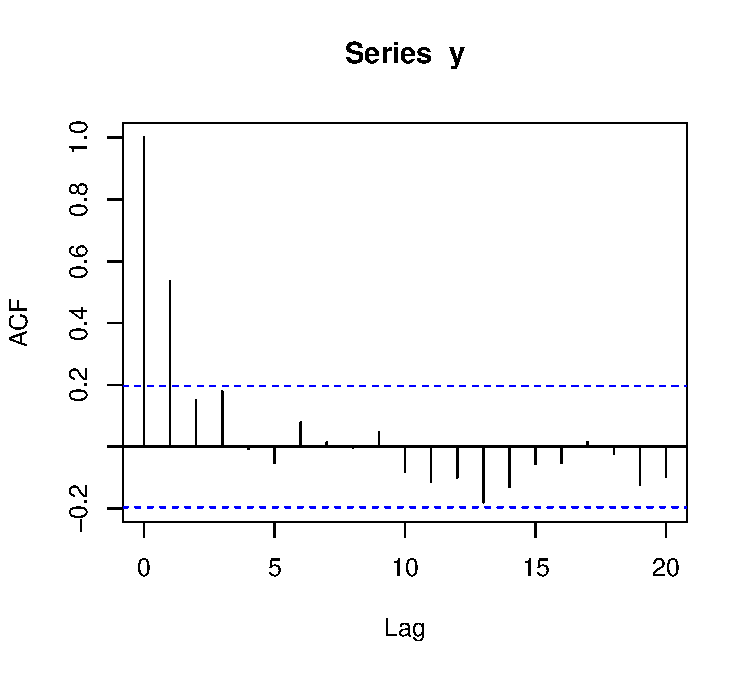
\includegraphics[width=\maxwidth]{figure/sassuolo-1} 

\end{knitrout}

As promised, everything beyond lag 1 is just chance.

\end{frame}

\begin{frame}[fragile]{AR process}
  
Another kind of time series is AR process, where each value depends on previous one, like this:

{\footnotesize
\begin{knitrout}
\definecolor{shadecolor}{rgb}{0.969, 0.969, 0.969}\color{fgcolor}\begin{kframe}
\begin{alltt}
\hlstd{e}\hlkwb{=}\hlkwd{rnorm}\hlstd{(}\hlnum{100}\hlstd{)}
\hlstd{x}\hlkwb{=}\hlkwd{numeric}\hlstd{(}\hlnum{0}\hlstd{)}
\hlstd{x[}\hlnum{1}\hlstd{]}\hlkwb{=}\hlnum{0}
\hlstd{alpha}\hlkwb{=}\hlnum{0.7}
\hlkwa{for} \hlstd{(i} \hlkwa{in} \hlnum{2}\hlopt{:}\hlnum{100}\hlstd{)}
\hlstd{\{}
  \hlstd{x[i]}\hlkwb{=}\hlstd{alpha}\hlopt{*}\hlstd{x[i}\hlopt{-}\hlnum{1}\hlstd{]}\hlopt{+}\hlstd{e[i]}
\hlstd{\}}
\hlstd{x}
\end{alltt}
\begin{verbatim}
##   [1]  0.00000000  0.69150384 -0.27156693 -1.69374385
##   [5] -0.04624706 -0.61289729  0.26464756 -0.21493841
##   [9] -1.31429232  0.44277420  0.09918044  0.19080999
##  [13] -1.02379326  0.16693770  0.98374525  0.04866219
##  [17]  1.22331904 -0.04784703 -0.21367820 -0.68228901
##  [21]  0.25079396 -0.86025292  1.75818244  1.19266409
##  [25]  0.30513461  2.41224530  1.28151011  1.68979182
##  [29]  2.01815565  3.53754507  1.85840920  2.32513921
##  [33]  1.77111656  2.12223993  0.91095776  1.58477201
##  [37]  2.08225425  1.09623045 -0.76369221 -0.70809836
##  [41] -1.84439667 -0.38985352 -1.04265756 -0.86988314
##  [45] -1.14485961 -3.18900426 -2.93376468 -2.16075858
##  [49] -1.59508681 -1.74905113 -3.13933449 -3.02637272
##  [53] -1.44218503 -1.55489860 -1.73928909 -2.00995900
##  [57] -2.66272165 -3.20337770 -3.51822345 -3.07147301
##  [61] -3.97833623 -3.76371790 -3.52532969 -3.45189431
##  [65] -0.06074526 -0.57178351  0.81558455 -0.27386449
##  [69]  0.75054673 -1.41070534 -2.60770962 -0.77008248
##  [73] -0.44599398  0.92659720 -0.50866042 -0.28000966
##  [77] -0.69941661 -0.87488058 -1.34524333 -1.24758120
##  [81] -2.20687436 -1.55318855 -0.03079664 -0.30483692
##  [85]  1.32564353  1.13381949  0.88141908  0.19972924
##  [89] -1.03973656 -0.60655913  0.27269352  0.49555143
##  [93]  0.74140308  0.41684887 -0.01247512 -0.08955967
##  [97]  1.09794055  0.51405840  1.27608083  0.05862015
\end{verbatim}
\end{kframe}
\end{knitrout}
}
  
\end{frame}

\begin{frame}[fragile]{Comments}
  
  \begin{itemize}
\item Each random shock now only used for its own value of \texttt{x}
\item but \texttt{x[i]} also depends on previous value \texttt{x[i-1]}
\item so correlated with previous value
\item but \texttt{x[i]} also contains multiple of \texttt{x[i-2]} and
  previous x's 
\item so all x's correlated, but autocorrelation dying away.

  \end{itemize}
  
\end{frame}

\begin{frame}[fragile]{ACF for AR(1) series}
  
\begin{knitrout}
\definecolor{shadecolor}{rgb}{0.969, 0.969, 0.969}\color{fgcolor}\begin{kframe}
\begin{alltt}
\hlkwd{acf}\hlstd{(x)}
\end{alltt}
\end{kframe}
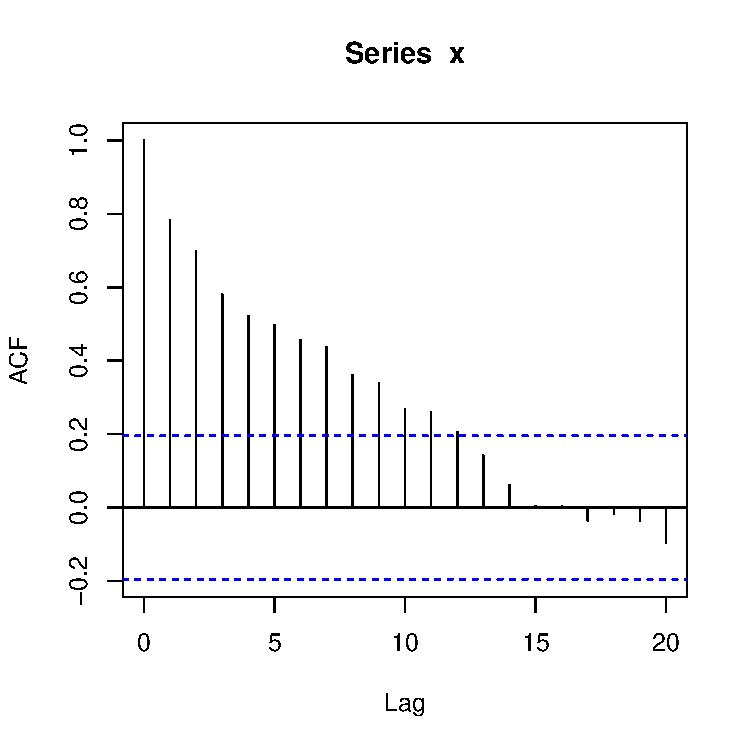
\includegraphics[width=\maxwidth]{figure/dssahasjhs-1} 

\end{knitrout}
  
\end{frame}

\begin{frame}[fragile]{Partial autocorrelation function}
  
This cuts off for an AR series.
The lag-2 autocorrelation should not be significant, and is only just:


\begin{knitrout}
\definecolor{shadecolor}{rgb}{0.969, 0.969, 0.969}\color{fgcolor}\begin{kframe}
\begin{alltt}
\hlkwd{pacf}\hlstd{(x)}
\end{alltt}
\end{kframe}
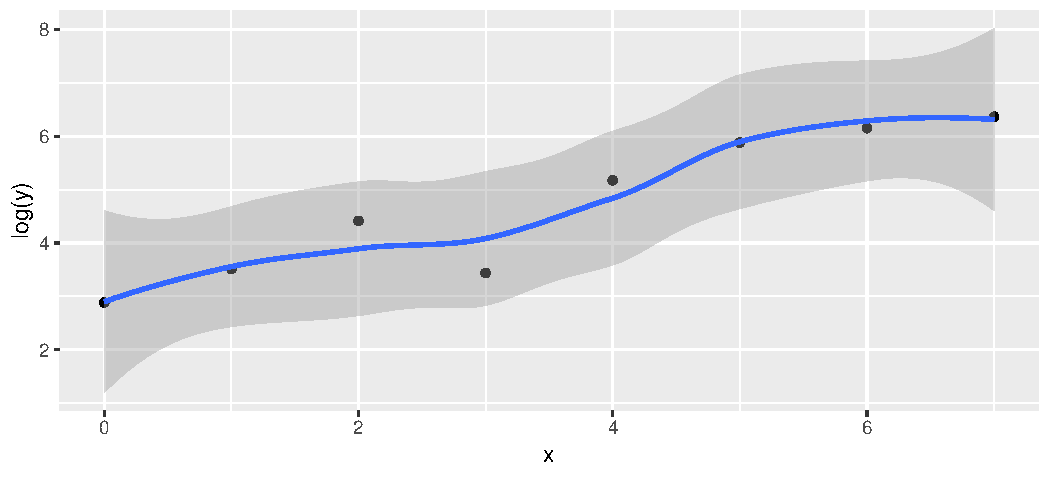
\includegraphics[width=\maxwidth]{figure/unnamed-chunk-26-1} 

\end{knitrout}
  
\end{frame}


\begin{frame}[fragile]{PACF for an MA series}
  
Decays slowly for an MA series:

\begin{knitrout}
\definecolor{shadecolor}{rgb}{0.969, 0.969, 0.969}\color{fgcolor}\begin{kframe}
\begin{alltt}
\hlkwd{pacf}\hlstd{(y)}
\end{alltt}
\end{kframe}
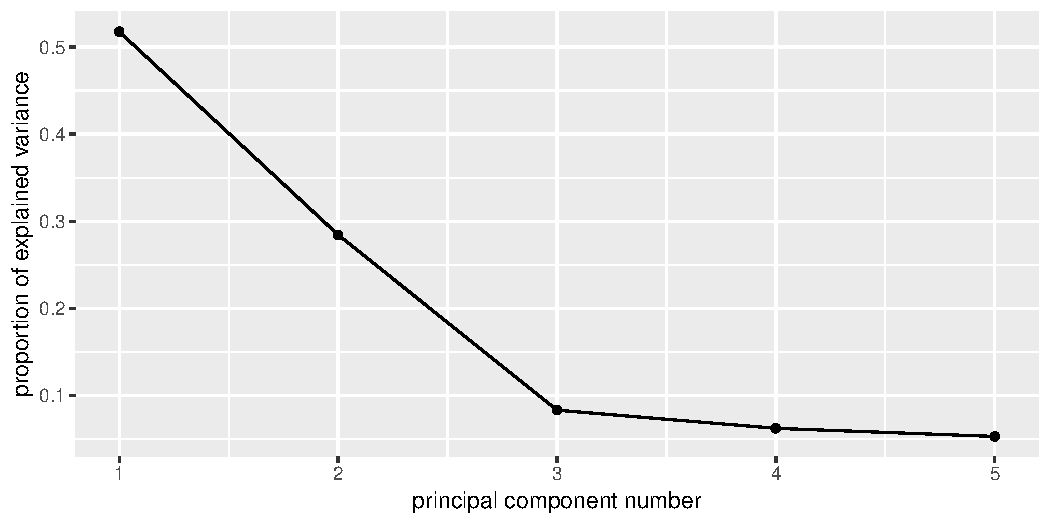
\includegraphics[width=\maxwidth]{figure/unnamed-chunk-27-1} 

\end{knitrout}
  
\end{frame}

\begin{frame}[fragile]{ACF for an MA series}
  
\begin{knitrout}
\definecolor{shadecolor}{rgb}{0.969, 0.969, 0.969}\color{fgcolor}\begin{kframe}
\begin{alltt}
\hlkwd{acf}\hlstd{(y)}
\end{alltt}
\end{kframe}
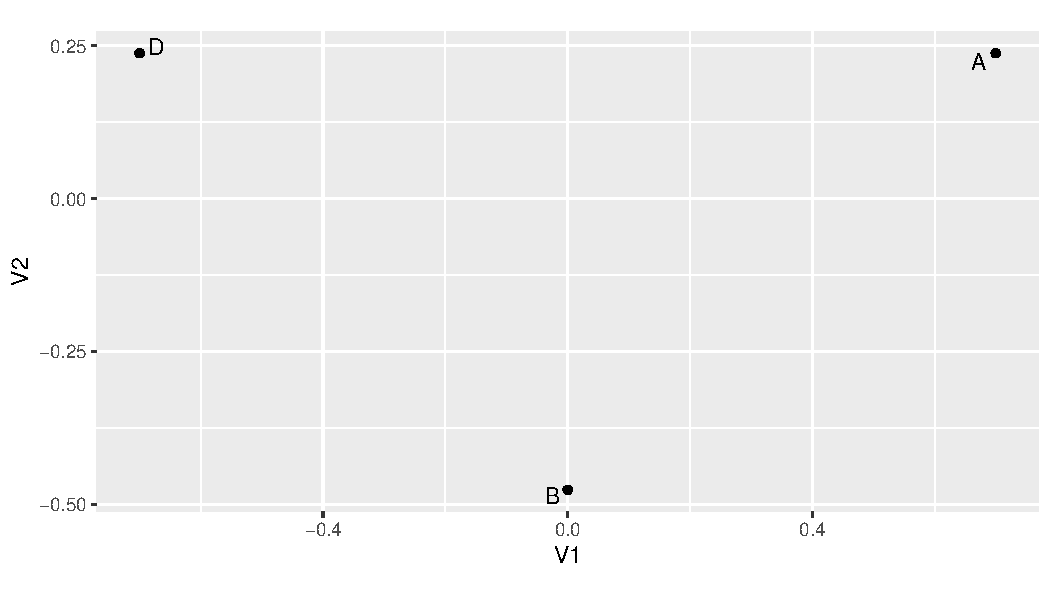
\includegraphics[width=\maxwidth]{figure/unnamed-chunk-28-1} 

\end{knitrout}
  
\end{frame}


\begin{frame}{The old way of doing time series analysis}
  
Starting from a series with constant variability (eg. transform first to get it, as for souvenirs):

\begin{itemize}
\item Assess stationarity.
\item If not stationary, take differences as many times as needed until it is.
\item Look at ACF, see if it dies off. If it does, you have MA series.
\item Look at PACF, see if that dies off. If it does, have AR series.
\item If neither dies off, probably have a mixed "ARMA" series.
\item Fit coefficients (like regression slopes).
\item Do forecasts.

\end{itemize}
  
\end{frame}

\begin{frame}[fragile]{The new way of doing time series analysis (in R)}
  
  \begin{itemize}
\item Transform series if needed to get constant variability
\item Use package \texttt{forecast}.
\item Use function \texttt{auto.arima} to estimate what kind of series
  best fits data. 
\item Use \texttt{forecast} to see what will happen in future.

  \end{itemize}
  
\end{frame}

\begin{frame}[fragile]{Load package \texttt{forecast}}
  
\begin{knitrout}
\definecolor{shadecolor}{rgb}{0.969, 0.969, 0.969}\color{fgcolor}\begin{kframe}
\begin{alltt}
\hlkwd{library}\hlstd{(forecast)}
\end{alltt}


{\ttfamily\noindent\itshape\color{messagecolor}{\#\# Loading required package: zoo}}

{\ttfamily\noindent\itshape\color{messagecolor}{\#\# \\\#\# Attaching package: 'zoo'}}

{\ttfamily\noindent\itshape\color{messagecolor}{\#\# The following objects are masked from 'package:base':\\\#\# \\\#\#\ \ \ \  as.Date, as.Date.numeric}}

{\ttfamily\noindent\itshape\color{messagecolor}{\#\# Loading required package: timeDate}}

{\ttfamily\noindent\itshape\color{messagecolor}{\#\# Loading required package: methods}}

{\ttfamily\noindent\itshape\color{messagecolor}{\#\# This is forecast 7.3}}\end{kframe}
\end{knitrout}
  
\end{frame}

\begin{frame}[fragile]{Anatomy of \texttt{auto.arima} output}

{\footnotesize  

\begin{knitrout}
\definecolor{shadecolor}{rgb}{0.969, 0.969, 0.969}\color{fgcolor}\begin{kframe}
\begin{alltt}
\hlkwd{auto.arima}\hlstd{(y)}
\end{alltt}
\begin{verbatim}
## Series: y 
## ARIMA(0,0,1) with zero mean     
## 
## Coefficients:
##          ma1
##       0.9070
## s.e.  0.0617
## 
## sigma^2 estimated as 0.9878:  log likelihood=-141.64
## AIC=287.29   AICc=287.41   BIC=292.5
\end{verbatim}
\end{kframe}
\end{knitrout}
}

\begin{itemize}
\item ARIMA part tells you what kind of series you are estimated to have:
\begin{itemize}
  \item first number (first 0) is AR (autoregressive) part
  \item second number (second 0) is amount of differencing here
  \item third number (1) is MA (moving average) part

\end{itemize}
  
\item Below that, coefficients (with SEs)
\item AICc is measure of fit (lower better)

\end{itemize}

\end{frame}

\begin{frame}[fragile]{What other models were possible?}
  
Run \texttt{auto.arima} with \texttt{trace=T}:

{\footnotesize
\begin{knitrout}
\definecolor{shadecolor}{rgb}{0.969, 0.969, 0.969}\color{fgcolor}\begin{kframe}
\begin{alltt}
\hlkwd{auto.arima}\hlstd{(y,}\hlkwc{trace}\hlstd{=T)}
\end{alltt}
\begin{verbatim}
## 
##  ARIMA(2,0,2) with non-zero mean : Inf
##  ARIMA(0,0,0) with non-zero mean : 345.2328
##  ARIMA(1,0,0) with non-zero mean : 313.9535
##  ARIMA(0,0,1) with non-zero mean : 287.9463
##  ARIMA(0,0,0) with zero mean     : 346.0889
##  ARIMA(1,0,1) with non-zero mean : 290.112
##  ARIMA(0,0,2) with non-zero mean : 290.1128
##  ARIMA(1,0,2) with non-zero mean : 291.7865
##  ARIMA(0,0,1) with zero mean     : 287.4124
##  ARIMA(1,0,1) with zero mean     : 289.4909
##  ARIMA(0,0,2) with zero mean     : 289.4993
##  ARIMA(1,0,2) with zero mean     : 290.6071
## 
##  Best model: ARIMA(0,0,1) with zero mean
## Series: y 
## ARIMA(0,0,1) with zero mean     
## 
## Coefficients:
##          ma1
##       0.9070
## s.e.  0.0617
## 
## sigma^2 estimated as 0.9878:  log likelihood=-141.64
## AIC=287.29   AICc=287.41   BIC=292.5
\end{verbatim}
\end{kframe}
\end{knitrout}
}

Also possible were MA(2) and ARMA(1,1), both with \texttt{AICc}=289.5.
  
  
\end{frame}

\begin{frame}[fragile]{Doing it all the new way: white noise}
  
\begin{knitrout}
\definecolor{shadecolor}{rgb}{0.969, 0.969, 0.969}\color{fgcolor}\begin{kframe}
\begin{alltt}
\hlstd{wn.aa}\hlkwb{=}\hlkwd{auto.arima}\hlstd{(wn.ts)}
\hlstd{wn.aa}
\end{alltt}
\begin{verbatim}
## Series: wn.ts 
## ARIMA(0,0,0) with zero mean     
## 
## sigma^2 estimated as 1.111:  log likelihood=-147.16
## AIC=296.32   AICc=296.36   BIC=298.93
\end{verbatim}
\end{kframe}
\end{knitrout}

Best fit \emph{is} white noise (no AR, no MA, no differencing). 

\end{frame}


\begin{frame}[fragile]{Forecasts}
  
{\small  
\begin{knitrout}
\definecolor{shadecolor}{rgb}{0.969, 0.969, 0.969}\color{fgcolor}\begin{kframe}
\begin{alltt}
\hlkwd{forecast}\hlstd{(wn.aa)}
\end{alltt}
\begin{verbatim}
##     Point Forecast     Lo 80    Hi 80     Lo 95    Hi 95
## 101              0 -1.350869 1.350869 -2.065975 2.065975
## 102              0 -1.350869 1.350869 -2.065975 2.065975
## 103              0 -1.350869 1.350869 -2.065975 2.065975
## 104              0 -1.350869 1.350869 -2.065975 2.065975
## 105              0 -1.350869 1.350869 -2.065975 2.065975
## 106              0 -1.350869 1.350869 -2.065975 2.065975
## 107              0 -1.350869 1.350869 -2.065975 2.065975
## 108              0 -1.350869 1.350869 -2.065975 2.065975
## 109              0 -1.350869 1.350869 -2.065975 2.065975
## 110              0 -1.350869 1.350869 -2.065975 2.065975
\end{verbatim}
\end{kframe}
\end{knitrout}
}

Forecasts all 0, since the past doesn't help to predict future.

\end{frame}

\begin{frame}[fragile]{MA(1)}
  
\begin{knitrout}
\definecolor{shadecolor}{rgb}{0.969, 0.969, 0.969}\color{fgcolor}\begin{kframe}
\begin{alltt}
\hlstd{y.aa}\hlkwb{=}\hlkwd{auto.arima}\hlstd{(y)}
\hlstd{y.aa}
\end{alltt}
\begin{verbatim}
## Series: y 
## ARIMA(0,0,1) with zero mean     
## 
## Coefficients:
##          ma1
##       0.9070
## s.e.  0.0617
## 
## sigma^2 estimated as 0.9878:  log likelihood=-141.64
## AIC=287.29   AICc=287.41   BIC=292.5
\end{verbatim}
\begin{alltt}
\hlstd{y.f}\hlkwb{=}\hlkwd{forecast}\hlstd{(y.aa)}
\end{alltt}
\end{kframe}
\end{knitrout}
  
\end{frame}

\begin{frame}[fragile]{Plotting the forecasts for MA(1)}
  
\begin{knitrout}
\definecolor{shadecolor}{rgb}{0.969, 0.969, 0.969}\color{fgcolor}\begin{kframe}
\begin{alltt}
\hlkwd{plot}\hlstd{(y.f)}
\end{alltt}
\end{kframe}
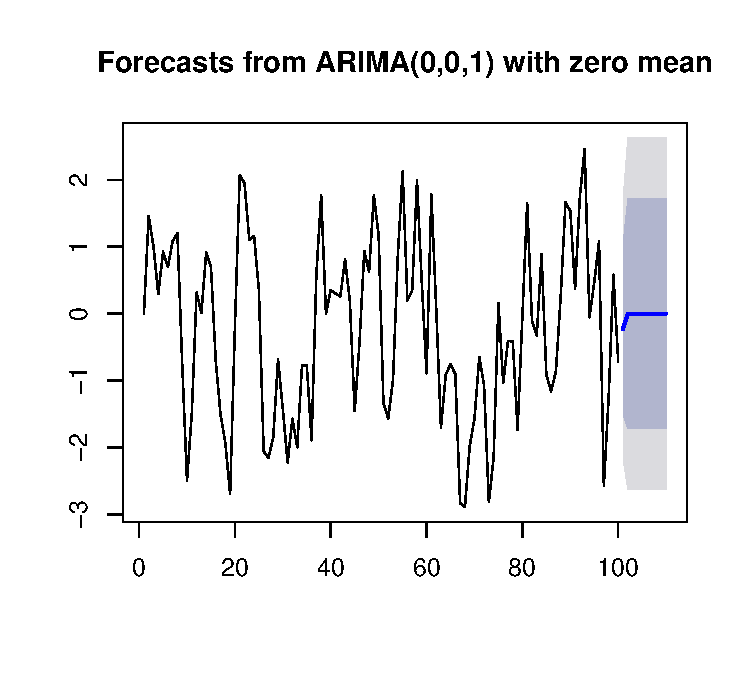
\includegraphics[width=\maxwidth]{figure/catanzaro-1} 

\end{knitrout}
  
\end{frame}

\begin{frame}[fragile]{AR(1)}
  
\begin{knitrout}
\definecolor{shadecolor}{rgb}{0.969, 0.969, 0.969}\color{fgcolor}\begin{kframe}
\begin{alltt}
\hlstd{x.aa}\hlkwb{=}\hlkwd{auto.arima}\hlstd{(x)}
\hlstd{x.aa}
\end{alltt}
\begin{verbatim}
## Series: x 
## ARIMA(0,1,1)                    
## 
## Coefficients:
##           ma1
##       -0.3544
## s.e.   0.1062
## 
## sigma^2 estimated as 0.979:  log likelihood=-138.99
## AIC=281.97   AICc=282.1   BIC=287.16
\end{verbatim}
\end{kframe}
\end{knitrout}
  
\end{frame}

\begin{frame}[fragile]{Oops!}
  
Got it wrong! Fit right AR(1) model:

\begin{knitrout}
\definecolor{shadecolor}{rgb}{0.969, 0.969, 0.969}\color{fgcolor}\begin{kframe}
\begin{alltt}
\hlstd{x.arima}\hlkwb{=}\hlkwd{arima}\hlstd{(x,}\hlkwc{order}\hlstd{=}\hlkwd{c}\hlstd{(}\hlnum{1}\hlstd{,}\hlnum{0}\hlstd{,}\hlnum{0}\hlstd{))}
\hlstd{x.arima}
\end{alltt}
\begin{verbatim}
## 
## Call:
## arima(x = x, order = c(1, 0, 0))
## 
## Coefficients:
##          ar1  intercept
##       0.7758    -0.3646
## s.e.  0.0611     0.4220
## 
## sigma^2 estimated as 0.957:  log likelihood = -140.16,  aic = 286.31
\end{verbatim}
\end{kframe}
\end{knitrout}

  
  
\end{frame}

\begin{frame}[fragile]{Forecasts for \texttt{x}}
  
\begin{knitrout}
\definecolor{shadecolor}{rgb}{0.969, 0.969, 0.969}\color{fgcolor}\begin{kframe}
\begin{alltt}
\hlkwd{plot}\hlstd{(}\hlkwd{forecast}\hlstd{(x.arima))}
\end{alltt}
\end{kframe}
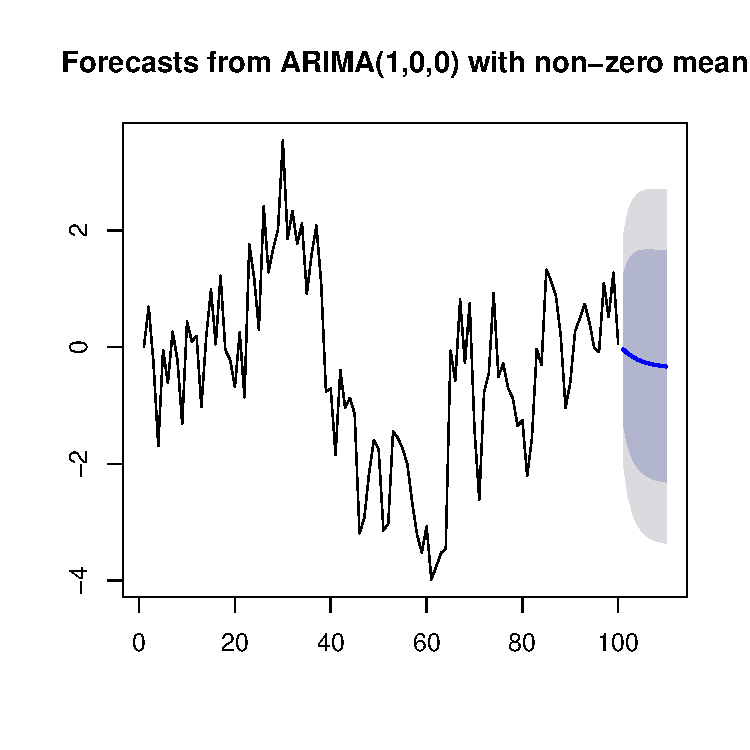
\includegraphics[width=\maxwidth]{figure/reggiana-1} 

\end{knitrout}
  
\end{frame}


\begin{frame}[fragile]{Comparing wrong model}
  
\begin{knitrout}
\definecolor{shadecolor}{rgb}{0.969, 0.969, 0.969}\color{fgcolor}\begin{kframe}
\begin{alltt}
\hlkwd{plot}\hlstd{(}\hlkwd{forecast}\hlstd{(x.aa))}
\end{alltt}
\end{kframe}
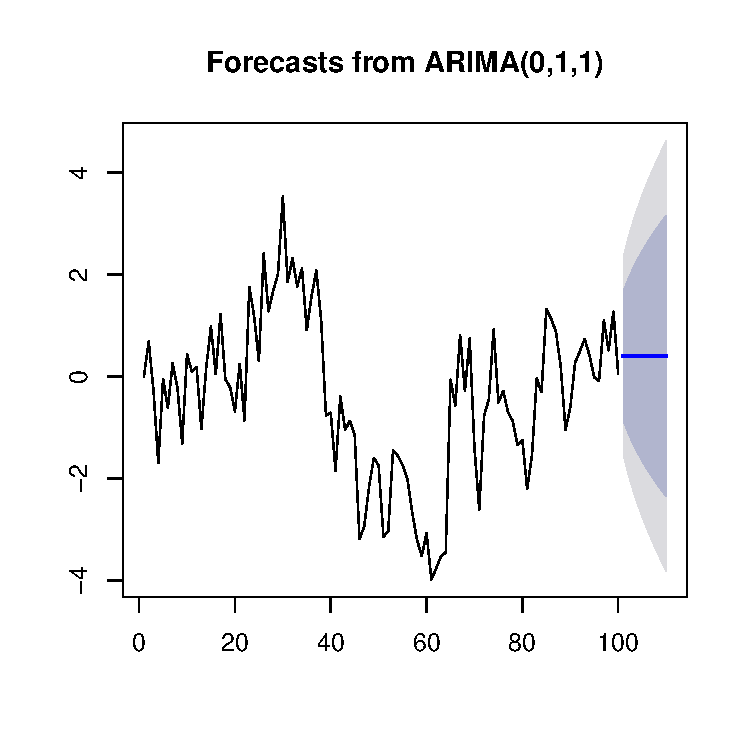
\includegraphics[width=\maxwidth]{figure/reggina-1} 

\end{knitrout}
  
\end{frame}

\begin{frame}[fragile]{Kings}
  
\begin{knitrout}
\definecolor{shadecolor}{rgb}{0.969, 0.969, 0.969}\color{fgcolor}\begin{kframe}
\begin{alltt}
\hlstd{kings.aa}\hlkwb{=}\hlkwd{auto.arima}\hlstd{(kings.ts)}
\hlstd{kings.aa}
\end{alltt}
\begin{verbatim}
## Series: kings.ts 
## ARIMA(0,1,1)                    
## 
## Coefficients:
##           ma1
##       -0.7218
## s.e.   0.1208
## 
## sigma^2 estimated as 236.2:  log likelihood=-170.06
## AIC=344.13   AICc=344.44   BIC=347.56
\end{verbatim}
\end{kframe}
\end{knitrout}
  
\end{frame}

\begin{frame}[fragile]{Kings forecasts}
  
\begin{knitrout}
\definecolor{shadecolor}{rgb}{0.969, 0.969, 0.969}\color{fgcolor}\begin{kframe}
\begin{alltt}
\hlstd{kings.f}\hlkwb{=}\hlkwd{forecast}\hlstd{(kings.aa)}
\hlstd{kings.f}
\end{alltt}
\begin{verbatim}
##    Point Forecast    Lo 80    Hi 80    Lo 95     Hi 95
## 43       67.75063 48.05479 87.44646 37.62845  97.87281
## 44       67.75063 47.30662 88.19463 36.48422  99.01703
## 45       67.75063 46.58489 88.91637 35.38042 100.12084
## 46       67.75063 45.88696 89.61429 34.31304 101.18822
## 47       67.75063 45.21064 90.29062 33.27869 102.22257
## 48       67.75063 44.55402 90.94723 32.27448 103.22678
## 49       67.75063 43.91549 91.58577 31.29793 104.20333
## 50       67.75063 43.29362 92.20763 30.34687 105.15439
## 51       67.75063 42.68718 92.81408 29.41939 106.08187
## 52       67.75063 42.09507 93.40619 28.51383 106.98742
\end{verbatim}
\end{kframe}
\end{knitrout}
  
\end{frame}

\begin{frame}[fragile]{Kings forecasts, plotted}
  
\begin{knitrout}
\definecolor{shadecolor}{rgb}{0.969, 0.969, 0.969}\color{fgcolor}\begin{kframe}
\begin{alltt}
\hlkwd{plot}\hlstd{(kings.f)}
\end{alltt}
\end{kframe}
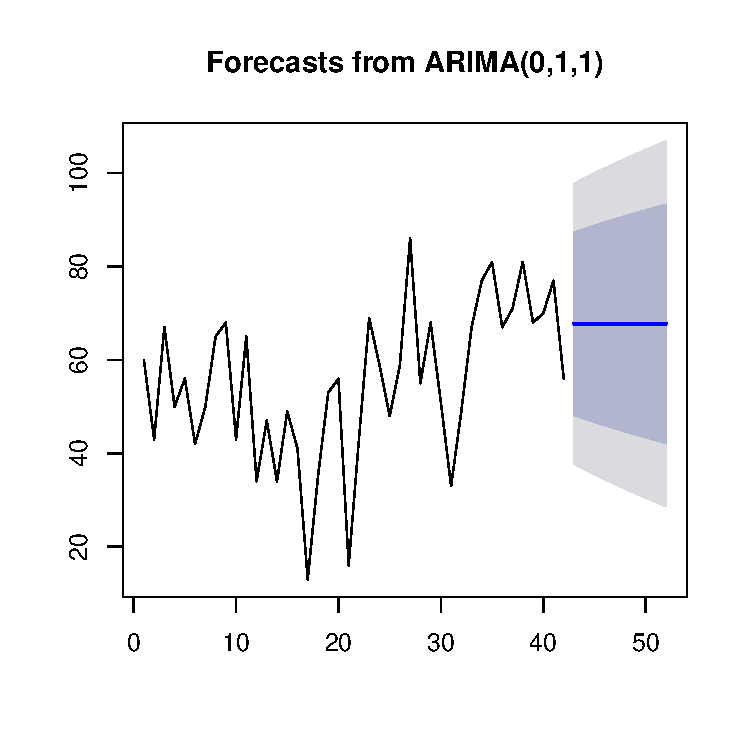
\includegraphics[width=\maxwidth]{figure/dob-1} 

\end{knitrout}
  
\end{frame}

\begin{frame}[fragile]{NY births}

\begin{knitrout}
\definecolor{shadecolor}{rgb}{0.969, 0.969, 0.969}\color{fgcolor}\begin{kframe}
\begin{alltt}
\hlstd{ny.aa}\hlkwb{=}\hlkwd{auto.arima}\hlstd{(ny.ts)}
\hlstd{ny.aa}
\end{alltt}
\begin{verbatim}
## Series: ny.ts 
## ARIMA(2,1,2)(1,1,1)[12]                    
## 
## Coefficients:
##          ar1      ar2      ma1     ma2     sar1     sma1
##       0.6539  -0.4540  -0.7255  0.2532  -0.2427  -0.8451
## s.e.  0.3003   0.2429   0.3227  0.2878   0.0985   0.0995
## 
## sigma^2 estimated as 0.4076:  log likelihood=-157.45
## AIC=328.91   AICc=329.67   BIC=350.21
\end{verbatim}
\begin{alltt}
\hlstd{ny.f}\hlkwb{=}\hlkwd{forecast}\hlstd{(ny.aa,}\hlkwc{h}\hlstd{=}\hlnum{36}\hlstd{)}
\end{alltt}
\end{kframe}
\end{knitrout}

Going 36 time periods (3 years) into future.

\end{frame}

\begin{frame}[fragile]{NY births forecasts}
  
Not \emph{quite} same every year:

{\small
\begin{knitrout}
\definecolor{shadecolor}{rgb}{0.969, 0.969, 0.969}\color{fgcolor}\begin{kframe}
\begin{alltt}
\hlstd{ny.f}\hlopt{$}\hlstd{mean}
\end{alltt}
\begin{verbatim}
##           Jan      Feb      Mar      Apr      May      Jun
## 1960 27.69056 26.07680 29.26544 27.59444 28.93193 28.55379
## 1961 27.66908 26.21255 29.22612 27.58011 28.71354 28.21736
## 1962 28.05431 26.55936 29.61570 27.96392 29.14695 28.67933
##           Jul      Aug      Sep      Oct      Nov      Dec
## 1960 29.84713 29.45347 29.16388 29.21343 27.26221 28.06863
## 1961 29.98728 29.96127 29.56515 29.54543 27.57845 28.40796
## 1962 30.33348 30.21822 29.84798 29.84511 27.88196 28.70585
\end{verbatim}
\end{kframe}
\end{knitrout}
}
  
\end{frame}


\begin{frame}[fragile]{Plotting the forecasts}

\begin{knitrout}
\definecolor{shadecolor}{rgb}{0.969, 0.969, 0.969}\color{fgcolor}\begin{kframe}
\begin{alltt}
\hlkwd{plot}\hlstd{(ny.f)}
\end{alltt}
\end{kframe}
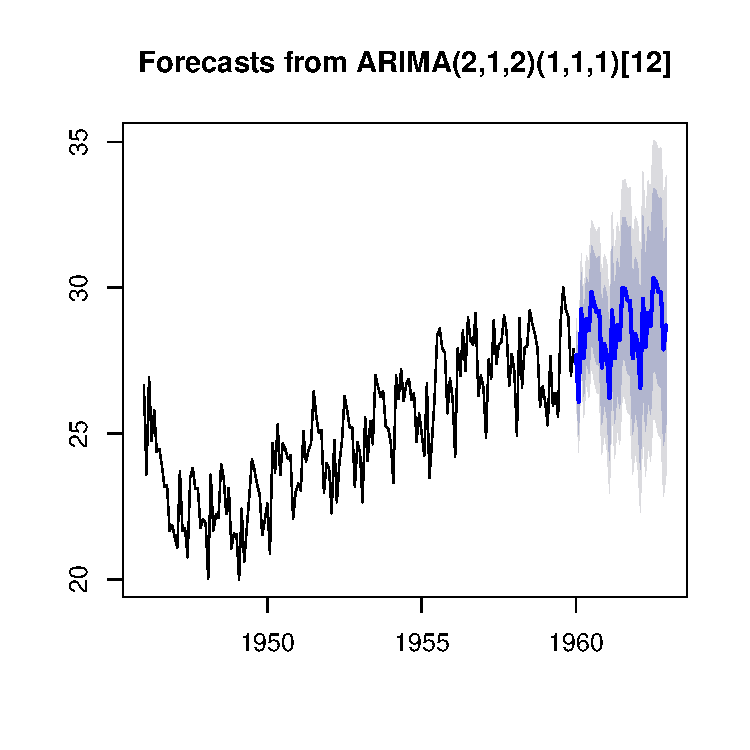
\includegraphics[width=\maxwidth]{figure/bradford-1} 

\end{knitrout}
  
\end{frame}

\begin{frame}[fragile]{Log-souvenir sales}
  
\begin{knitrout}
\definecolor{shadecolor}{rgb}{0.969, 0.969, 0.969}\color{fgcolor}\begin{kframe}
\begin{alltt}
\hlstd{souv.aa}\hlkwb{=}\hlkwd{auto.arima}\hlstd{(souv.log.ts)}
\hlstd{souv.aa}
\end{alltt}
\begin{verbatim}
## Series: souv.log.ts 
## ARIMA(2,0,0)(1,1,0)[12] with drift         
## 
## Coefficients:
##          ar1     ar2     sar1   drift
##       0.3493  0.3602  -0.3278  0.0247
## s.e.  0.1086  0.1159   0.1334  0.0044
## 
## sigma^2 estimated as 0.03004:  log likelihood=23.04
## AIC=-36.09   AICc=-35.18   BIC=-24.71
\end{verbatim}
\begin{alltt}
\hlstd{souv.f}\hlkwb{=}\hlkwd{forecast}\hlstd{(souv.aa,}\hlkwc{h}\hlstd{=}\hlnum{27}\hlstd{)}
\end{alltt}
\end{kframe}
\end{knitrout}
  
\end{frame}

\begin{frame}[fragile]{The forecasts}

Differenced series showed low value for January (large drop). December
highest, Jan and Feb lowest. Forecast actual sales, not log sales:

{\footnotesize
\begin{knitrout}
\definecolor{shadecolor}{rgb}{0.969, 0.969, 0.969}\color{fgcolor}\begin{kframe}
\begin{alltt}
\hlkwd{exp}\hlstd{(souv.f}\hlopt{$}\hlstd{mean)}
\end{alltt}
\begin{verbatim}
##            Jan       Feb       Mar       Apr       May
## 1994  14202.53  16488.11  28958.71  22967.17  20163.96
## 1995  18961.56  21616.41  39190.18  31099.30  27735.03
## 1996  25572.45  29326.17  52616.13                    
##            Jun       Jul       Aug       Sep       Oct
## 1994  24862.41  33805.66  37909.52  42014.85  43083.67
## 1995  33539.58  46100.67  51257.10  56101.66  57245.39
## 1996                                                  
##            Nov       Dec
## 1994  63766.10 142925.27
## 1995  85335.26 191340.89
## 1996
\end{verbatim}
\end{kframe}
\end{knitrout}
}
  
\end{frame}

\begin{frame}[fragile]{Plotting the forecasts}
  
\begin{knitrout}
\definecolor{shadecolor}{rgb}{0.969, 0.969, 0.969}\color{fgcolor}\begin{kframe}
\begin{alltt}
\hlkwd{plot}\hlstd{(souv.f)}
\end{alltt}
\end{kframe}
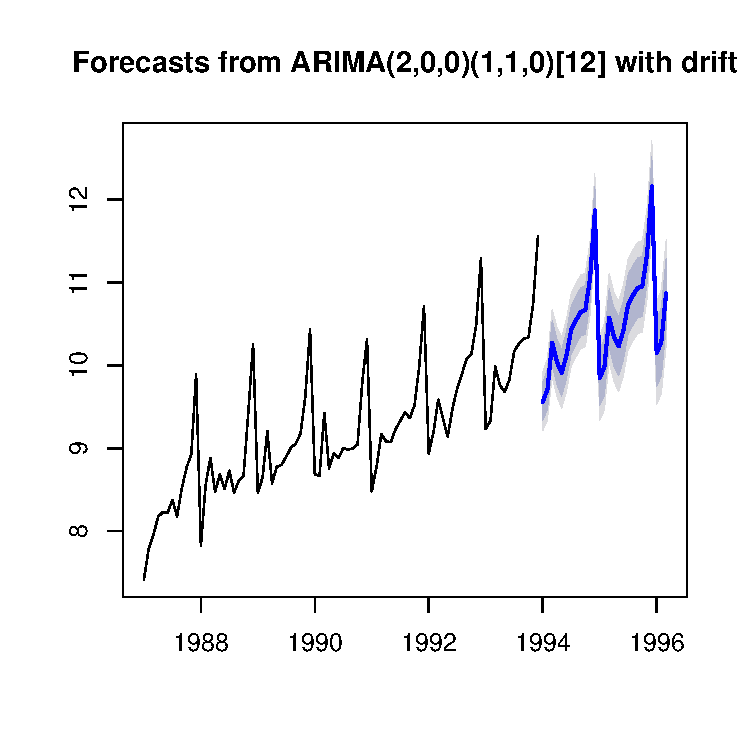
\includegraphics[width=\maxwidth]{figure/castleford-1} 

\end{knitrout}
  
\end{frame}

\begin{frame}[fragile]{Global mean temperatures, revisited}
  
\begin{knitrout}
\definecolor{shadecolor}{rgb}{0.969, 0.969, 0.969}\color{fgcolor}\begin{kframe}
\begin{alltt}
\hlkwd{attach}\hlstd{(temp)}
\hlstd{temp.ts}\hlkwb{=}\hlkwd{ts}\hlstd{(temperature,}\hlkwc{start}\hlstd{=}\hlnum{1880}\hlstd{)}
\hlstd{temp.aa}\hlkwb{=}\hlkwd{auto.arima}\hlstd{(temp.ts)}
\hlstd{temp.aa}
\end{alltt}
\begin{verbatim}
## Series: temp.ts 
## ARIMA(3,1,2) with drift         
## 
## Coefficients:
##           ar1      ar2      ar3     ma1      ma2   drift
##       -0.6899  -0.0517  -0.2748  0.2235  -0.5436  0.0066
## s.e.   0.1566   0.1904   0.1052  0.1529   0.1520  0.0028
## 
## sigma^2 estimated as 0.008872:  log likelihood=125.31
## AIC=-236.62   AICc=-235.71   BIC=-216.55
\end{verbatim}
\end{kframe}
\end{knitrout}
  
\end{frame}

\begin{frame}[fragile]{Forecasts}
  
\begin{knitrout}
\definecolor{shadecolor}{rgb}{0.969, 0.969, 0.969}\color{fgcolor}\begin{kframe}
\begin{alltt}
\hlstd{temp.f}\hlkwb{=}\hlkwd{forecast}\hlstd{(temp.aa)}
\hlkwd{plot}\hlstd{(temp.f)}
\end{alltt}
\end{kframe}
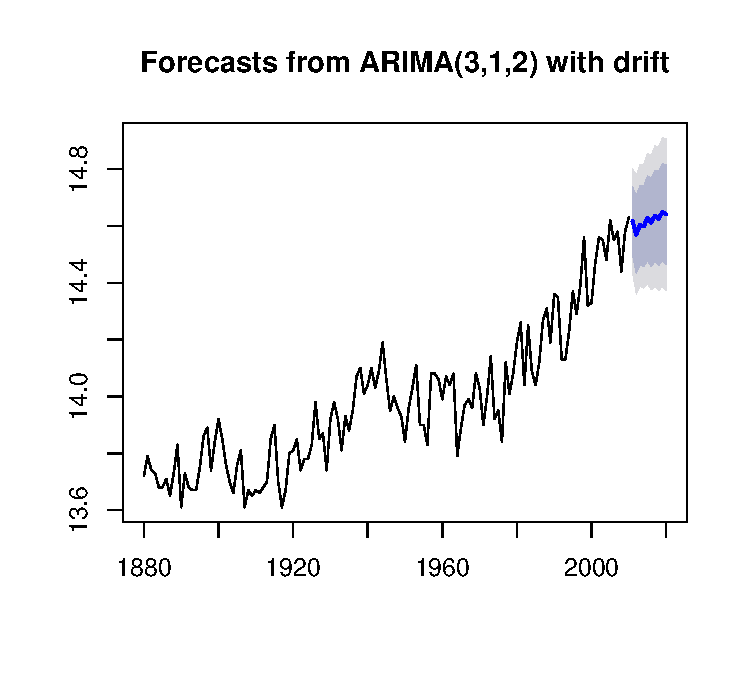
\includegraphics[width=\maxwidth]{figure/wakefield-1} 

\end{knitrout}
\end{frame}
